\chapter{Resultados}
\comentarioM{Escribir todo en presente!!!!}
\section{Experimentación}
Con el objetivo de elegir los métodos definitivos usados en cada etapa de cada sistema de seguimiento se realizaron varias pruebas. En esta sección explicaremos cuales fueron estas pruebas, cómo se eligieron los valores para los distintos parámetros de cada método y mostraremos los resultados de los métodos elegidos, tanto para RGB como para Depth. También analizaremos el funcionamiento del sistema de seguimiento RGB-D.

Para lograr una buena comparación entre métodos de seguimiento cuadro a cuadro, tanto para RGB como para Depth, utilizamos como método de detección el método ``ideal''. El mismo consta simplemente de tomar los datos provistos por el \textit{ground truth} para los frames en donde se requería correr una detección. En el caso de RGB los datos son tomados directamente desde el ground truth. Como la base de datos solo provee la ubicación del objeto en RGB en el caso de la detección en Depth estos datos se toman como punto de partida y luego se los refina tomando los datos del modelo 3D del objeto a buscar.

\subsection{Elección del método de seguimiento RGB}
Durante el proceso de selección de métodos se corrieron pruebas preeliminares para elegir aquellos que mejor se adaptaran a las escenas y objetos elegidos para este fin. Una vez hecho un primer filtro, se exploraron algunos parámetros de cada método para obtener los mejores valores de cada uno y luego hacer una selección final entre aquellos que mejor se desempeñaran. En esta sección explicaremos cuales fueron los métodos y cómo llegamos a elegir el definitivo.

Para el seguimiento RGB se tuvieron en cuenta dos métodos distintos. El primero utiliza SURF \cite{surf} para obtener puntos de interés y descriptores y luego un comparador para hacer comparaciones cuadro a cuadro. El segundo método consiste en extraer el histograma de la imagen RGB y utilizar un comparador de histogramas para hacer el seguimiento.

El método que mejor se desempeñó en las pruebas preeliminares es el basado en histogramas por lo que se exploraron distintas soluciones basadas en este método utilizando ahora las escenas tomadas de la base de datos. Este método tiene distintas variables a explorar:
\begin{itemize}
	\item Modelo de color: RGB o HSV y canales a utilizar de cada uno
	\item Cantidad de categorías/celdas del histograma
	\item Método de comparación de histogramas: \textit{Bhattachayyra}, \textit{Chi-Squared}, \textit{Correlation}, \textit{Intersection}
	\item Umbrales para las distancias frame a frame y template a frame
\end{itemize}


\begin{figure}
	\centering
	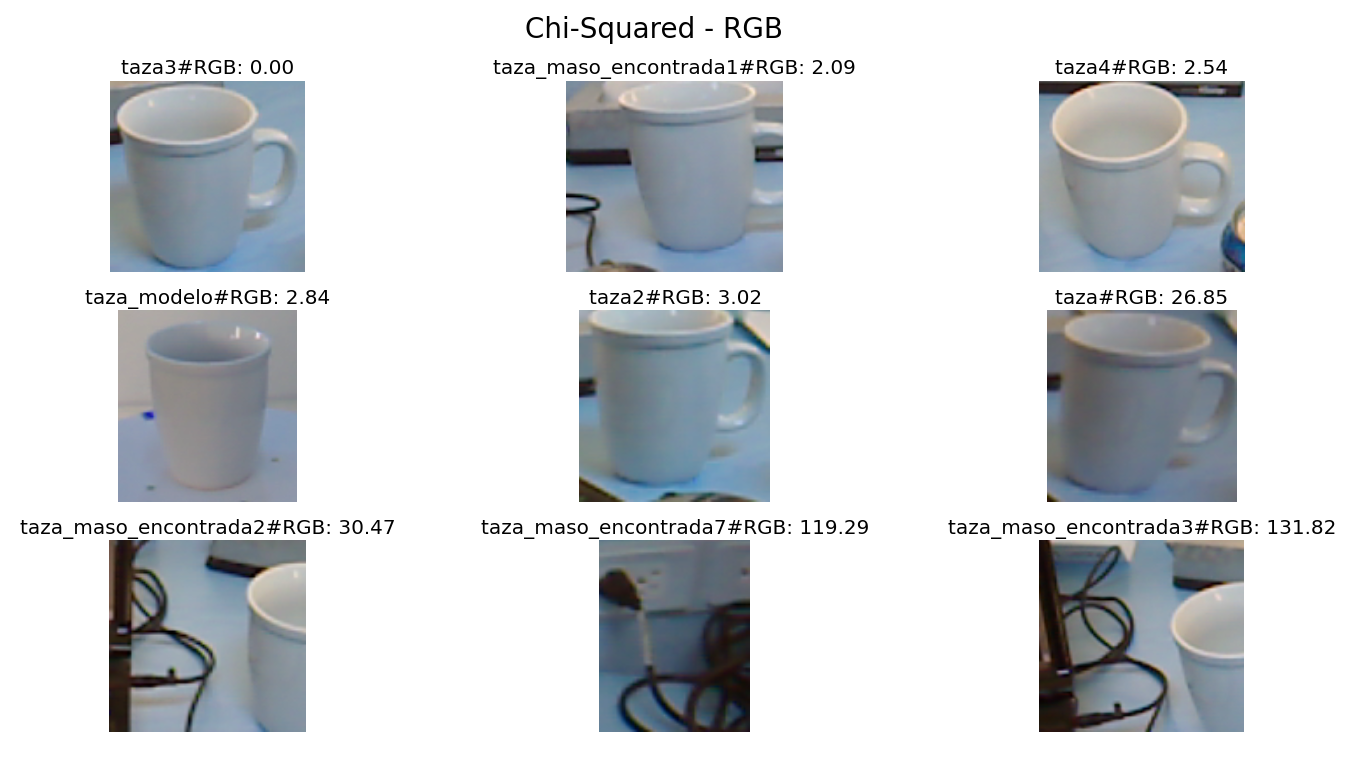
\includegraphics[width=\textwidth]{img/results_chi-squared_rgb_16r_4g_4b.png}
	\caption{Ordenando muestras según comparación por chi-squared, tomando los canales RGB, 16 bines para el canal rojo y 4 para el verde y el azul. El modelo utilizado es un template de la taza sacado de la escena.}
	\label{pruebas_eleccion_canales}
\end{figure}

Para decidir qué esquema de colores, qué canales y cuántas categorías por canal se iban a utilizar se eligieron dos objetos representativos de la base con sus respectivas escenas y se tomaron muestras de cada uno junto con muestras de distintas texturas de la escena o del mismo objeto pero en donde se lo veía de manera parcial. Una vez tomadas las muestras se eligió una como template/modelo del objeto y se realizó una comparación entre el modelo y las distintas muestras tomadas de la escena y se ordenaron de menor a mayor distancia. Esto se hizo fijando un método de comparación de histogramas. Un ejemplo de esto se puede ver en la Figura \ref{pruebas_eleccion_canales}. Esto se hizo con el objetivo de saber qué combinación de esquema, canales y bines por canal clasificaba mejor a las muestras.

De este análisis surgió que las mejores combinaciones de esquema, canales y bines para estos ejemplos fueron utilizar el canal verde en el caso de RGB con unos 60 bines, los 3 canales RGB con 8 bines por canal y los canales SV del esquema de colores HSV, con 8 y 16 bines respectivamente. Una vez reducido el espectro de posibilidades comenzamos a realizar pruebas con el fin de definir para cada uno de estos esquemas qué método de comparación de histogramas convenía utilizar y con qué valor de umbral se obtenian mejores resultados.

Para cuantificar la efectividad y robustes del tracking de cada algoritmo elegido decidimos evaluar las siguientes variables:
\begin{itemize}
	\item Promedio de área solapada: promedio de solapamiento de área, usando el cálculo propuesto en \cite{everinghampascal}, entre el objeto reportado por el algoritmo y el ground truth durante toda la escena teniendo en cuenta únicamente los casos en que se usó el algoritmo de seguimiento.
	\item Porcentaje de seguimiento: de todas las veces que el objeto aparece en la escena obtenemos el porcentaje de veces que el algoritmo de seguimiento fue exitoso, es decir que lo reporta como encontrado y el área reportada se solapa con el área reportada por el ground truth en al menos un 30\%
	\item Porcentaje de falsos positivos: cantidad de veces que el algoritmo reporta haber encontrado el objeto cuando en realidad no está en la imagen
	\item Porcentaje de falsos negativos: cantidad de veces que el algoritmo no encuentra el objeto cuando en realidad el mismo está en la imagen o que lo encuentra pero el área reportada se solapa en menos de un 30\% con el área reportada por el ground truth
\end{itemize}

Los mejores resultados que obtuvimos se pueden observar en las tablas \ref{pruebas_definitivas_bhatta_green}, \ref{pruebas_definitivas_correl_green} y \ref{pruebas_definitivas_rgb_sv}.

\begin{table}[h]
	\begin{tabular}{|c|c|c|c|c|c|}
	    \hline
	    & \multirow{2}{2.4cm}{\% promedio de overlap} & \multirow{2}{2cm}{\% veces seguido} & \multirow{2}{1.6cm}{\% Falsos Positivos} & \multirow{2}{1.6cm}{\% Falsos Negativos}\\
		Objeto & & & &\\
	    \hline
	    Taza   & 19.30      & 26.32   & 0       & 46.94 \\
	    \hline
	    Gorra  & 49.10      & 87.80   & 0       & 0     \\
	    \hline
	    Bowl   & 14.14      &  4.55   & 0       & 20    \\
	    \hline
    \end{tabular}
	\caption{Mejores resultados usando comparación de histogramas por Bhattachayyra para el canal verde con 60 bines}
	\label{pruebas_definitivas_bhatta_green}
\end{table}

\begin{table}[h]
	\begin{tabular}{|c|c|c|c|c|c|}
	    \hline
	    & \multirow{2}{2.4cm}{\% promedio de overlap} & \multirow{2}{2cm}{\% veces seguido} & \multirow{2}{1.6cm}{\% Falsos Positivos} & \multirow{2}{1.6cm}{\% Falsos Negativos}\\
		Objeto & & & &\\
	    \hline
	    Taza   & 14.83      & 13.16     & 0      & 58.16 \\
	    \hline
	    Gorra  & 49.14      & 95.12     & 0      & 1.02  \\
	    \hline
	    Bowl   & 17.47      & 13.64     & 5.26   & 26.84 \\
	    \hline
    \end{tabular}
	\caption{Mejores resultados usando comparación de histogramas por Correlation para el canal verde con 60 bines}
	\label{pruebas_definitivas_correl_green}
\end{table}

\begin{table}[h]
	\begin{tabular}{|c|c|c|c|c|c|}
	    \hline
	    & \multirow{2}{2.4cm}{\% promedio de overlap} & \multirow{2}{2cm}{\% veces seguido} & \multirow{2}{1.6cm}{\% Falsos Positivos} & \multirow{2}{1.6cm}{\% Falsos Negativos}\\
		Objeto & & & &\\
	    \hline
	    Taza   & 34.48      & 47.89     & 0        & 31.63  \\
	    \hline
	    Gorra  & 55.68      & 96.97     & 0        & 0      \\
	    \hline
	    Bowl   & 12.58      &  6.19     & 0        & 13.68  \\
	    \hline
    \end{tabular}
	\caption{Mejores resultados combinando comparación de histogramas por Bhattachayyra para RGB y para SV (del esquema HSV)}
	\label{pruebas_definitivas_rgb_sv}
\end{table}



\subsection{Evaluación del tracking RGB}\label{eval_rgb}
A continuación se muestran los resultados del algoritmo de seguimiento elegido para las imágenes RGB con los valores de los parámetros ya fijados. Para todas las pruebas se eligieron tres objetos distintos que aparecen en dos escenas, todos sacados de la base de datos indicada en la sección \ref{base_rgbd}.

Como podemos ver en la Tabla \ref{pruebas_definitivas_rgb_sv} el tracking se comporta de manera muy diversa dependiendo del objeto que se esté analizando. En los ejemplos de la taza y la gorra el algoritmo reporta haber encontrado al objeto en la mayoría de los casos, 85\% y 78\% respectivamente.\comentarioM{Acá me habias puesto un comentario que decía: ¿Qué significa?. Creo que ahora está un poco más claro escrito.} Este valor en conjunto con el promedio de solapamiento pueden darnos un indicio de que tan bien se desempeña el algoritmo. Si observamos el promedio de solapamiento vemos el algoritmo se comporta mucho mejor en el caso de la gorra, con un promedio de solapamiento del 55\%. Creemos que esto se debe a la marcada diferencia de color entre la gorra y el fondo de la imagen. Esto no sucede en el caso de la taza en el que repetidas veces el color de fondo varía entre colores y tonos similares a los de esta lo que provoca que la comparación de histogramas no sea robusta. En el caso del bowl el promedio de solapamiento es alto pero se debe a que el porcentaje de veces que se siguió al objeto es bajo. Como el algoritmo de detección es el ideal, cuantas más veces se usa la detección mejor es el porcentaje de solapamiento. Notamos que en esta escena los cambios de intensidad y textura son muy notorios lo que afecta negativamente al algoritmo.


\begin{figure}
	\centering
	\begin{subfigure}[b]{\textwidth}
		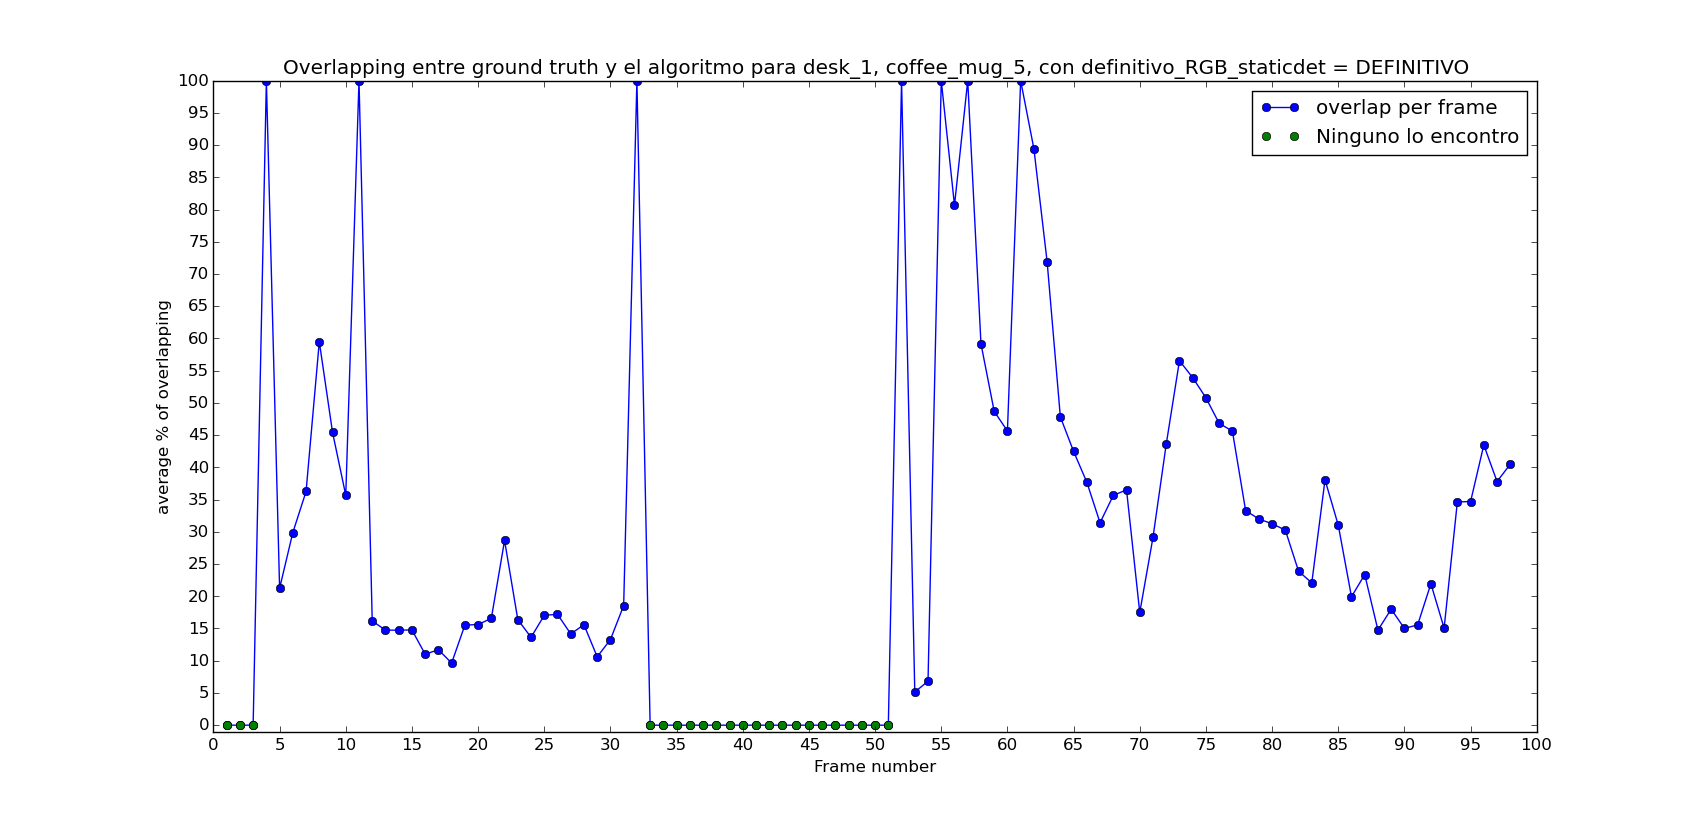
\includegraphics[width=\textwidth]{img/frame_a_frame/rgb-taza.png}
		\caption{Seguimiento frame a frame para la taza}
		\label{frame_frame_rgb_taza}
	\end{subfigure}
	\quad
	\begin{subfigure}[b]{\textwidth}
		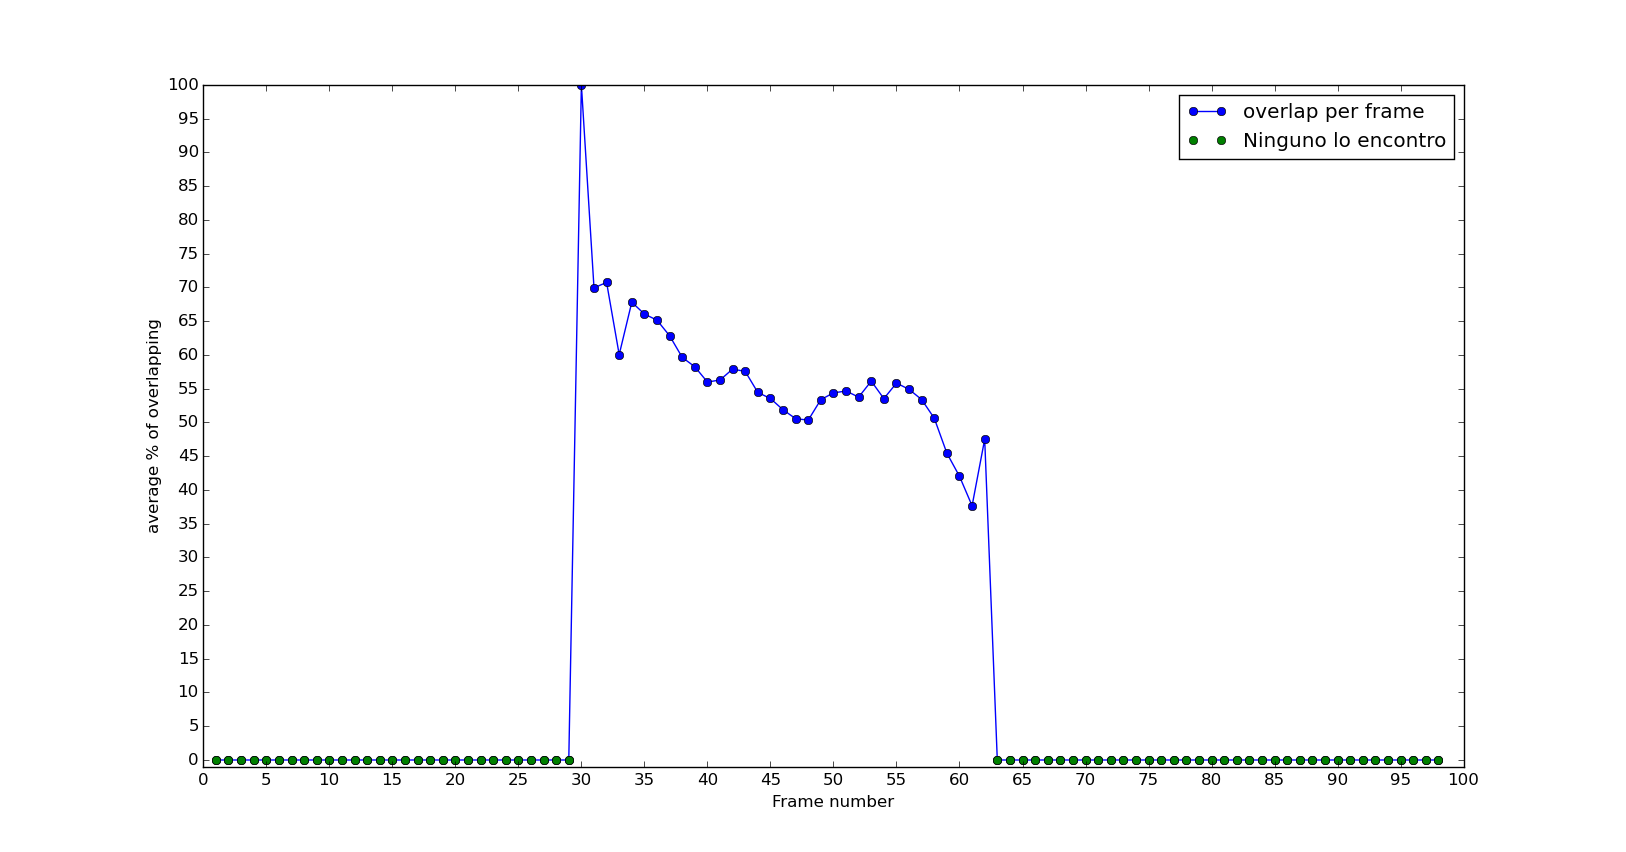
\includegraphics[width=\textwidth]{img/frame_a_frame/rgb-gorra.png}
		\caption{Seguimiento frame a frame para la gorra}
		\label{frame_frame_rgb_gorra}
	\end{subfigure}
	\quad
	\begin{subfigure}[b]{\textwidth}
		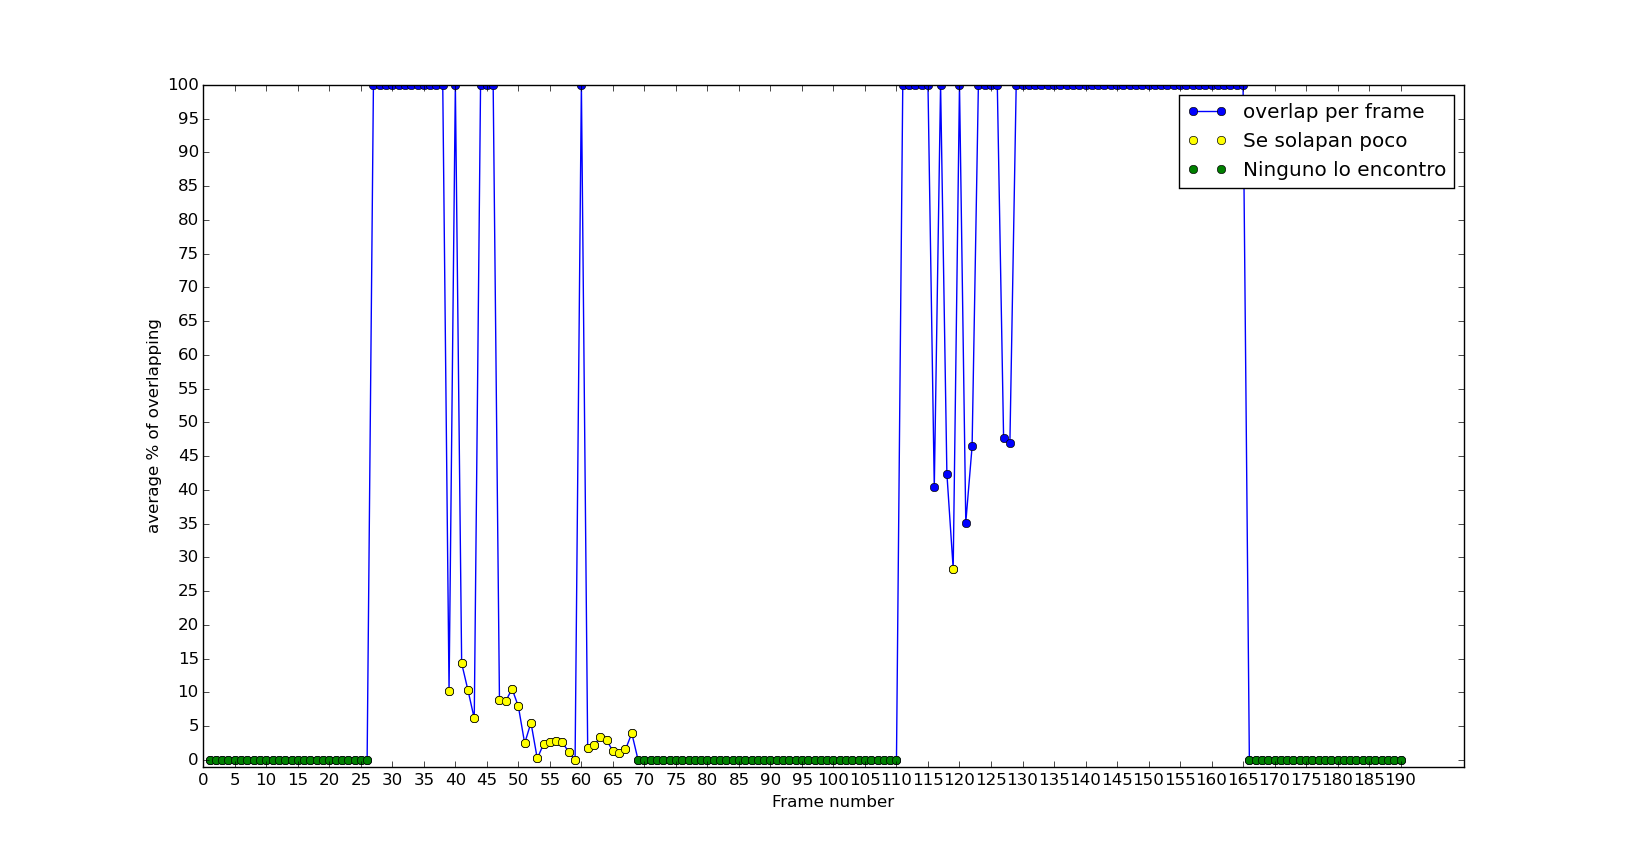
\includegraphics[width=\textwidth]{img/frame_a_frame/rgb-bowl.png}
		\caption{Seguimiento frame a frame para el bowl}
		\label{frame_frame_rgb_bowl}
	\end{subfigure}
	\caption{Seguimiento frame a frame del tracking RGB con detección ideal.}
	\label{frame_frame_rgb}
\end{figure}

En la Figura \ref{frame_frame_rgb} se visualiza mejor el comportamiento del algoritmo para cada objeto en las distintas escenas. En cada subfigura se muestra para cada escena y por cada frame el porcentaje de solapamiento entre el área del objeto reportada por el algoritmo y la indicada por el ground truth, siguiendo la métrica de Pascal VOC \cite{everinghampascal}. 

\customsubsubsection{Colores en los gráficos de seguimiento frame a frame}
Los colores en los puntos del gráfico representan los distintos resultados registrados por cada frame. Si el punto es de color verde, significa que el resultado reportado por nuestro algoritmo coincide con el ground truth en que el objeto no se encuentra en ese frame, es decir, es un verdadero negativo. Si el color es amarillo, significa que el algoritmo reportó haber encontrado al objeto y así también lo hace el ground truth, pero que las áreas reportadas no se solapan entre sí o el porcentaje de solapamiento es menor al 30\%. En este caso es un falso negativo. Pero también diferenciamos otro tipo de falso negativo, y se hace con el color naranja, y se usa cuando nuestro algoritmo no reporta haber encontrado al objeto pero el ground truth indica que el obtejo está en el frame.

Otro color que puede aparecer en este tipo de gráficos es el color rojo. El rojo indica un falso positivo, es decir, cuando el ground truth indica que el objeto no está en el frame y nuestro algoritmo reporta lo contrario. Además, también está el color azul. Este color indica que el resultado reportado por nuestro algoritmo se solapa en un 30\% o más con el área indicada por el ground truth. A diferencia del resto de los colores antes mencionados que aparecen todos sobre el 0 del eje de porcentaje de solapamiento, los puntos azules pueden aparecer a cualquier nivel de este eje. La altura en donde esté el punto azul indica el porcentaje de solapamiento para ese frame.








Finalmente, existe un color más que puede aparecer: el negro. Como se explicó en la Sección \ref{metodo_rgbd}, algunos de los algoritmos usados tienen un cierto grado de aleatoriedad. 

























Los puntos que están en 0 (color verde) indican que el objeto no fue encontrado y coincide con el ground truth, como es el caso de las subfiguras \ref{frame_frame_rgb_taza} y \ref{frame_frame_rgb_gorra}. En la subfigura \ref{frame_frame_rgb_bowl} se ven dos puntos en 0 de color amarillo. Esto indica que el algoritmo reporta haber seguido al objeto pero que el área no se solapa con el área del ground truth. Para las tres subfiguras, todos los frames cuyo área es igual a 100\% se corresponde con las veces que el algoritmo de detección fue corrido, es decir, cuando falló el seguimiento.

Se puede ver en el gráfico \ref{frame_frame_rgb_taza} que el algoritmo de seguimiento reporta un área que se solapa entre un 15\% y un 50\% en la mayoría de los casos. En el gráfico \ref{frame_frame_rgb_gorra} la mayoría oscila entre un 35\% y un 50\% y en el gráfico \ref{frame_frame_rgb_bowl} se observa que la mayoría se encuentra entre un 1\% y un 10\%. Una posible esxplicación de esto es que el algoritmo no funciona correctamente cuando los objetos tienen poca textura y esto empeora si existen objetos cercanos cuya textura sea similar a la del objeto que se está buscando. Este sería el caso de la taza y del bowl. Ambos son objetos con poca textura de color blanco que pueden camuflarse con otros objetos de la escena.

\subsection{Evaluación del tracking en profundidad}
En esta sección se muestran los resultados de ICP para las imágenes de profundidad (Depth) con los valores de los parámetros fijados. Para todas las pruebas se eligieron los mismos tres objetos que para el caso de la evaluación del tracking RGB (ver sección \ref{eval_rgb}).

\begin{table}[h]
    \begin{tabular}{|c|c|c|c|c|c|}
    \hline
    & \multirow{2}{2.4cm}{\% promedio de overlap} & \multirow{2}{2cm}{\% veces seguido} & \multirow{2}{1.6cm}{\% Falsos Positivos} & \multirow{2}{1.6cm}{\% Falsos Negativos}\\
	Objeto & & & &\\
    \hline
    Taza   & 66.29      & 92.16      & 0      & 0     \\
    \hline
    Gorra  & 56.85      & 92.67      & 0      & 0     \\
    \hline
    Bowl   & 40.60      & 63.83      & 4.74   & 14.39 \\
    \hline
    \end{tabular}
\caption{Resultados del tracking Depth utilizando como detección los valores sacados de la base de datos más una etapa de refinamiento de estos datos usando AP e ICP.}
\label{tabla_d}
\end{table}

En la Tabla \ref{tabla_d} se puede ver que el tracking se comporta de mejor manera que el algoritmo de RGB. Los tres ejemplos tienen una alta tasa de seguimiento. Además, en los tres casos se tiene un buen balance entre el promedio de solapamiento del área encontrada y el área reportada por el \textit{ground truth} y desvío estándar.

\begin{figure}
	\centering
	\begin{subfigure}[b]{\textwidth}
		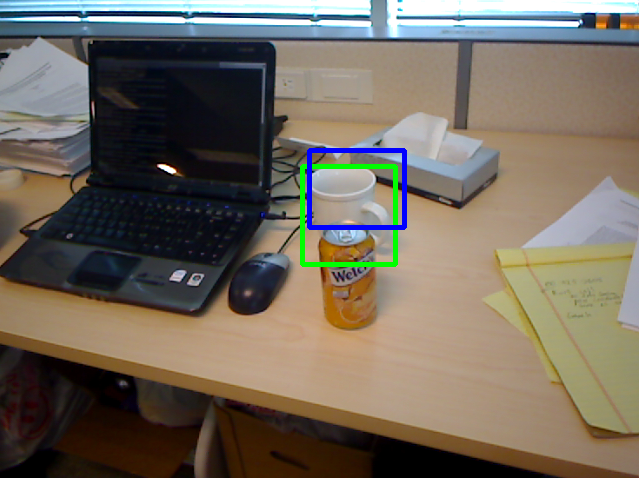
\includegraphics[width=\textwidth]{img/frame_98_taza_rgb.png}
		\caption{Seguimiento reportado por el tracking en Depth y proyectado en RGB.}
		\label{taza_ocluida_rgb}
	\end{subfigure}
	\quad
	\begin{subfigure}[b]{\textwidth}
		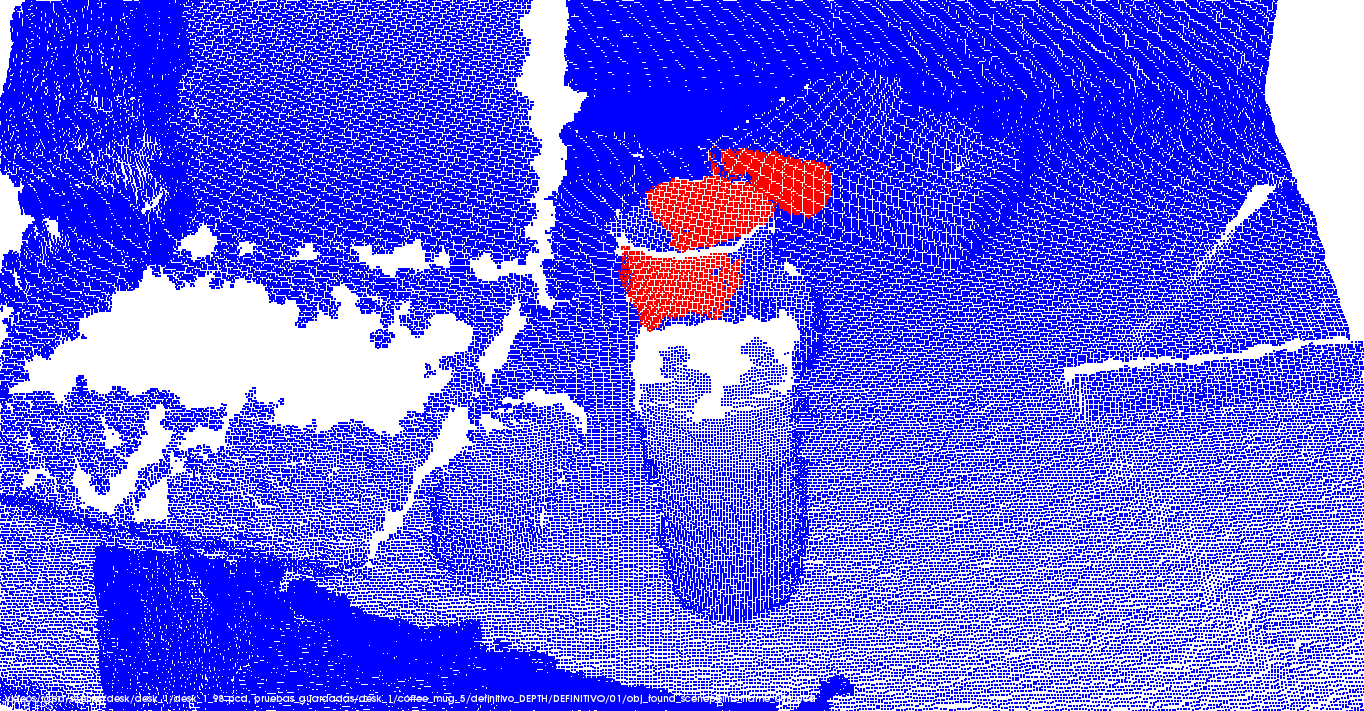
\includegraphics[width=\textwidth]{img/frame_98_taza_pcd.png}
		\caption{Visualización de la nube de puntos reportada por el tracking en Depth}
		\label{taza_ocluida_pcd}
	\end{subfigure}
	\caption{Muestra de un resultado del seguimiento en Depth. Las áreas se solapan en un 47\%.}
	\label{taza_ocluida}
\end{figure}

Un problema que encontramos en nuestra solución es que no hacemos un ajuste del tamaño del área reportada si el objeto está ocluído. En la Figura \ref{taza_ocluida} podemos ver como el algoritmo detecta de manera exitosa a la taza pero que solo reporta el área de la taza que está visible y no ajusta el tamaño al del modelo del objeto que se obtuvo en la etapa de entrenamiento. La subfigura \ref{taza_ocluida_rgb} muestra en color azul el recuadro reportado por nuestro algoritmo de seguimiento en donde se encuentra la taza. El recuadro verde corresponde al área que indica el ground truth como correcta. Se puede observar que el recuadro verde incluye además de la parte visible de la taza una porción importante de la lata que está delante de ella y que si se tiene en cuenta el tamaño de la taza esta área está incluyendo a la parte de la taza que se encuentra ocluida. A pesar de no ser algo que suceda reiteradas veces en las escenas y objetos elegidos para estas pruebas, puede ser un punto de mejora para nuestro algoritmo. \comentarioM{¿Digo algo de Kalman acá?}

Otra decisión que se tomó al implementar nuestro algoritmo fue no utilizar el modelo del objeto para refinar el seguimiento, por ejemplo, para realizar el filtrado de puntos de la escena que corresponden al objeto que se busca. Esto se debe a que dependiendo de la forma del objeto, de su pose en el frame actual y de su pose en el modelo no resulta sencillo decidir si es conveniente utilizar el modelo para hacer este filtrado. En cambio, decidimos utilizar la nube de puntos hallada en el frame anterior como base para filtrar los puntos en el frame actual una vez que se quiera refinar el resultado. Por este motivo es que en ocaciones el algoritmo devuelve como parte del resultado puntos que no corresponden al objeto que se busca.

En la imagen \ref{taza_ocluida_pcd} se pueden ver tres regiones de puntos de color rojo. Esas regiones son las reportadas por el algoritmo como puntos de la taza. Si las enumeramos de arriba hacia abajo, la primera región no forma parte de la taza sino que es parte de la caja de pañuelos que está detrás de la misma. Esto podría evitarse si se filtraran los puntos de la escena usando el modelo de la taza pero sólo porque la forma de la misma es simétrica (si no se tiene en cuenta su asa). En el caso de la gorra en cambio ya no queda tan claro que sirva filtrar usando el modelo porque la visera la hace asimétrica y el tamaño de la misma no permite despreciar esos puntos.

Haciendo un análisis de los frames anteriores al de la Figura \ref{taza_ocluida} y de cómo se fue desarrollando el seguimiento notamos que el motivo por el cual se incluye parte de la caja de pañuelos como puntos de la taza es porque en la etapa de detección falló el refinamiento por AP, ICP y el filtrado de puntos. En la Figura \ref{filtro_en_deteccion} mostramos como se ve una detección sacada directa desde la base de datos (subfigura \ref{filtro_en_deteccion_mal}) y un refinado de la detección (subfigura \ref{filtro_en_deteccion_bien} utilizando el modelo del objeto y alineándolo usando AP e ICP y filtrando los puntos de la escena.

\begin{figure}
	\centering
	\begin{subfigure}[b]{\textwidth}
		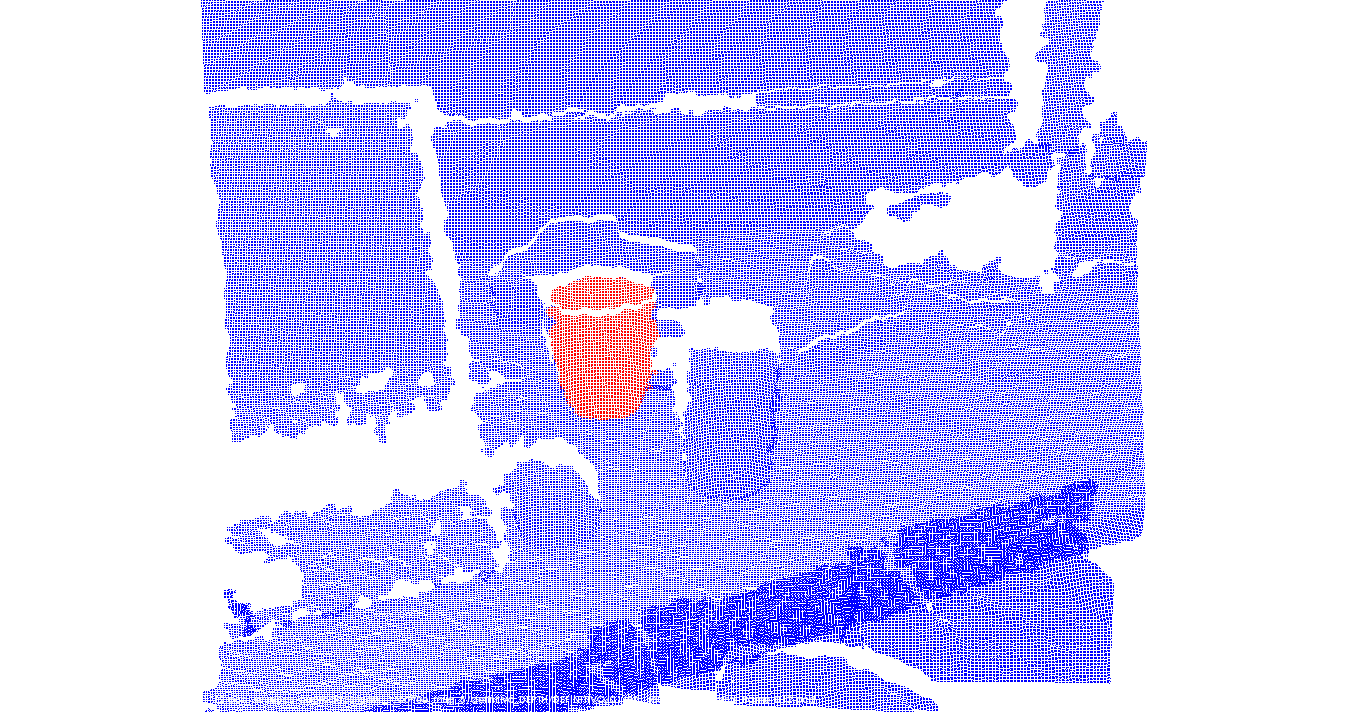
\includegraphics[width=\textwidth]{img/taza_filtrado_exitoso_definitivo_depth_frame12.png}
		\caption{Filtrado exitoso}
		\label{filtro_en_deteccion_bien}
	\end{subfigure}
	\quad
	\begin{subfigure}[b]{\textwidth}
		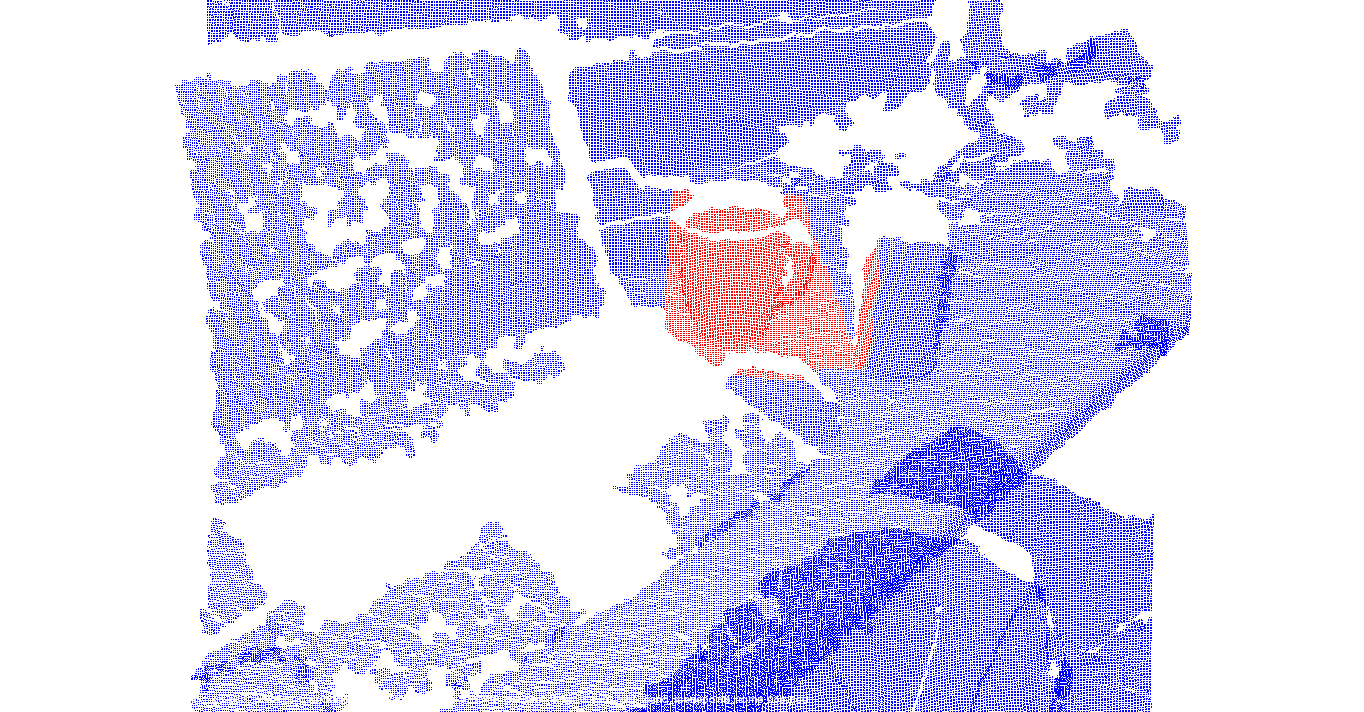
\includegraphics[width=\textwidth]{img/taza_filtrado_fallido_depth_simil_thresh_01_frame66.png}
		\caption{Filtrado fallido}
		\label{filtro_en_deteccion_mal}
	\end{subfigure}
	\caption{Nube de puntos de la taza filtrados de la escena}
	\label{filtro_en_deteccion}
\end{figure}

En la Figura \ref{frame_frame_d} se muestran para cada escena y objeto como se comportó el tracking frame a frame. El análisis es el mismo que se explicó para la Figura \ref{frame_frame_rgb}, aunque en estos gráficos aparecen algunas referencias nuevas. En la subfigura \ref{frame_frame_d_taza} se observan dos puntos de color naranja con valor 0\%. Estos valores corresponden a los frames 32 y 52. Estos puntos indican que el algoritmo de tracking reportó no encontrar al objeto cuando en realidad el objeto está en la imagen según los datos del ground truth. Estos puntos se corresponden con los dos falsos negativos reportados en la Tabla \ref{tabla_d} para la taza. En la Figura \ref{frame_frame_d_gorra} se puede identificar un punto rojo correspondiente al frame 66 con un valor del 0\%. Lo que indica este color es que el algoritmo de tracking reportó haber encontrado al objeto pero el ground truth indica que el objeto no se encuentra en ese frame, es decir, es un falso positivo. Por último, en la Figura \ref{frame_frame_d_bowl} existen múltiples puntos de color negro. Estos puntos indican que en las múltiples corridas del algoritmo para esta escena y con estos valores de parámetros hubo distintos resultados para el mismo frame. \comentarioP{Por qué? Explicar lo de random de AP} Entre los frames 72 y 108 el ground truth indica que el bowl no se encuentra en la escena. Los puntos negros en el gráfico \ref{frame_frame_d_bowl} entre dichos frames con valor 0\% indican que alguna de las corridas el algoritmo reportó haber encontrado al objeto, es decir que hubo falsos positivos y en otras reportó correctamente que el objeto no se hallaba en esos frames. Luego, entre los frames 109 y 122 además de haber puntos negros con valor 0\% existen algunos con valores mayormente cercanos al 15\%. Eso significa que en alguna de las corridas el algoritmo reportó haber encontrado al objeto y en otras no lo encontró en cuyo caso fueron falsos negativos. Lo que buscamos con este análisis es reducir la cantidad de puntos negros al mínimo ya que es un indicador de que tan robusto es el algoritmo.

\begin{figure}
	\centering
	\begin{subfigure}[b]{\textwidth}
		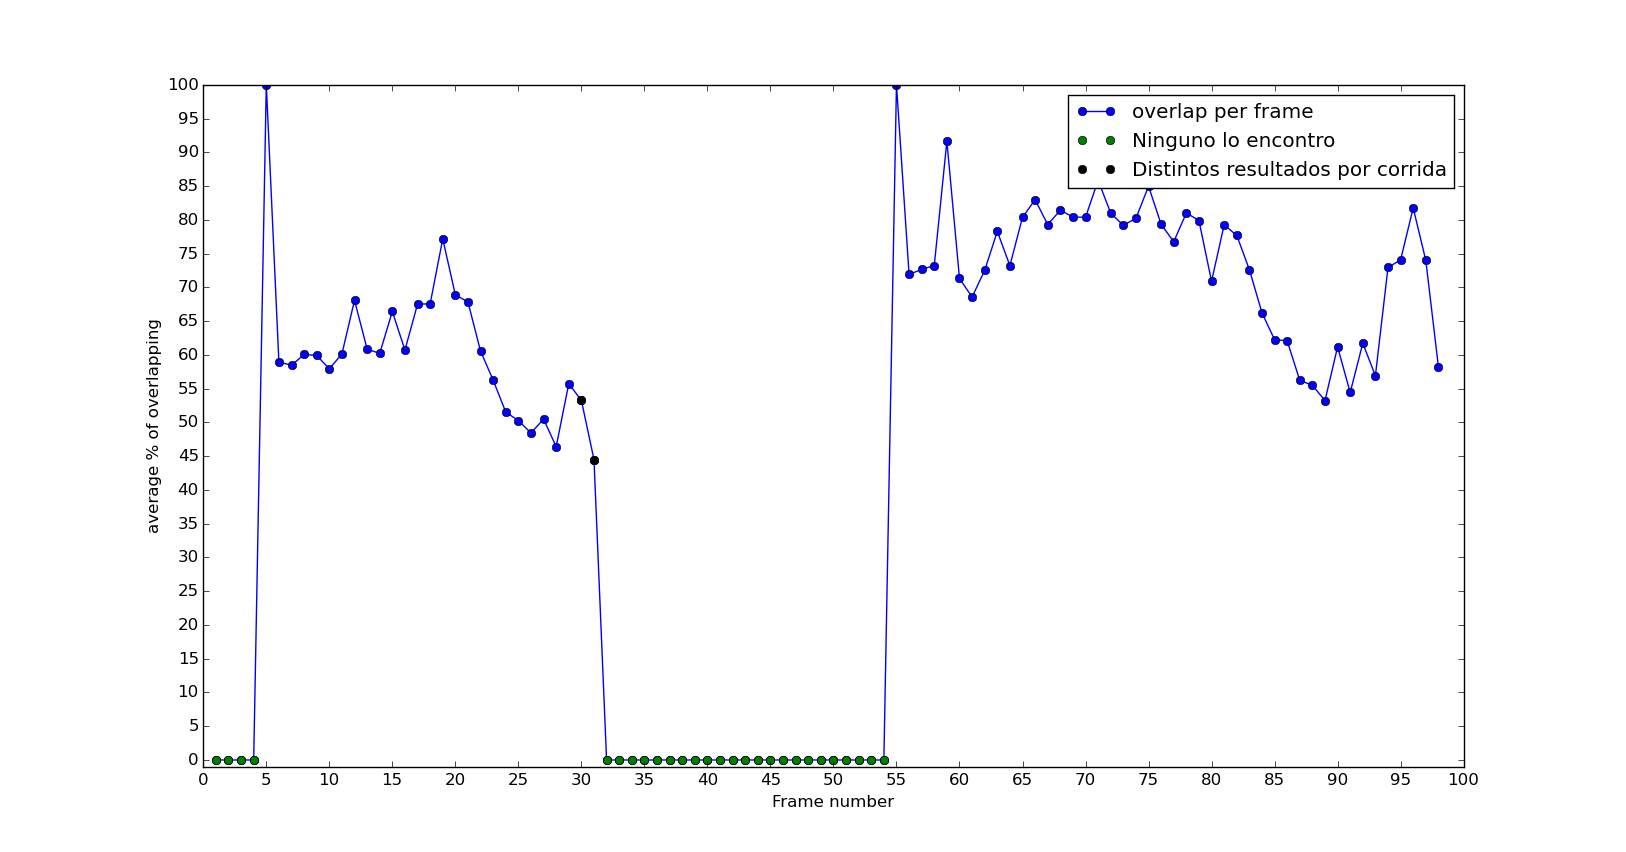
\includegraphics[width=\textwidth]{img/frame_a_frame/depth-taza.png}
		\caption{Seguimiento frame a frame para la taza}
		\label{frame_frame_d_taza}
	\end{subfigure}
	\quad
	\begin{subfigure}[b]{\textwidth}
		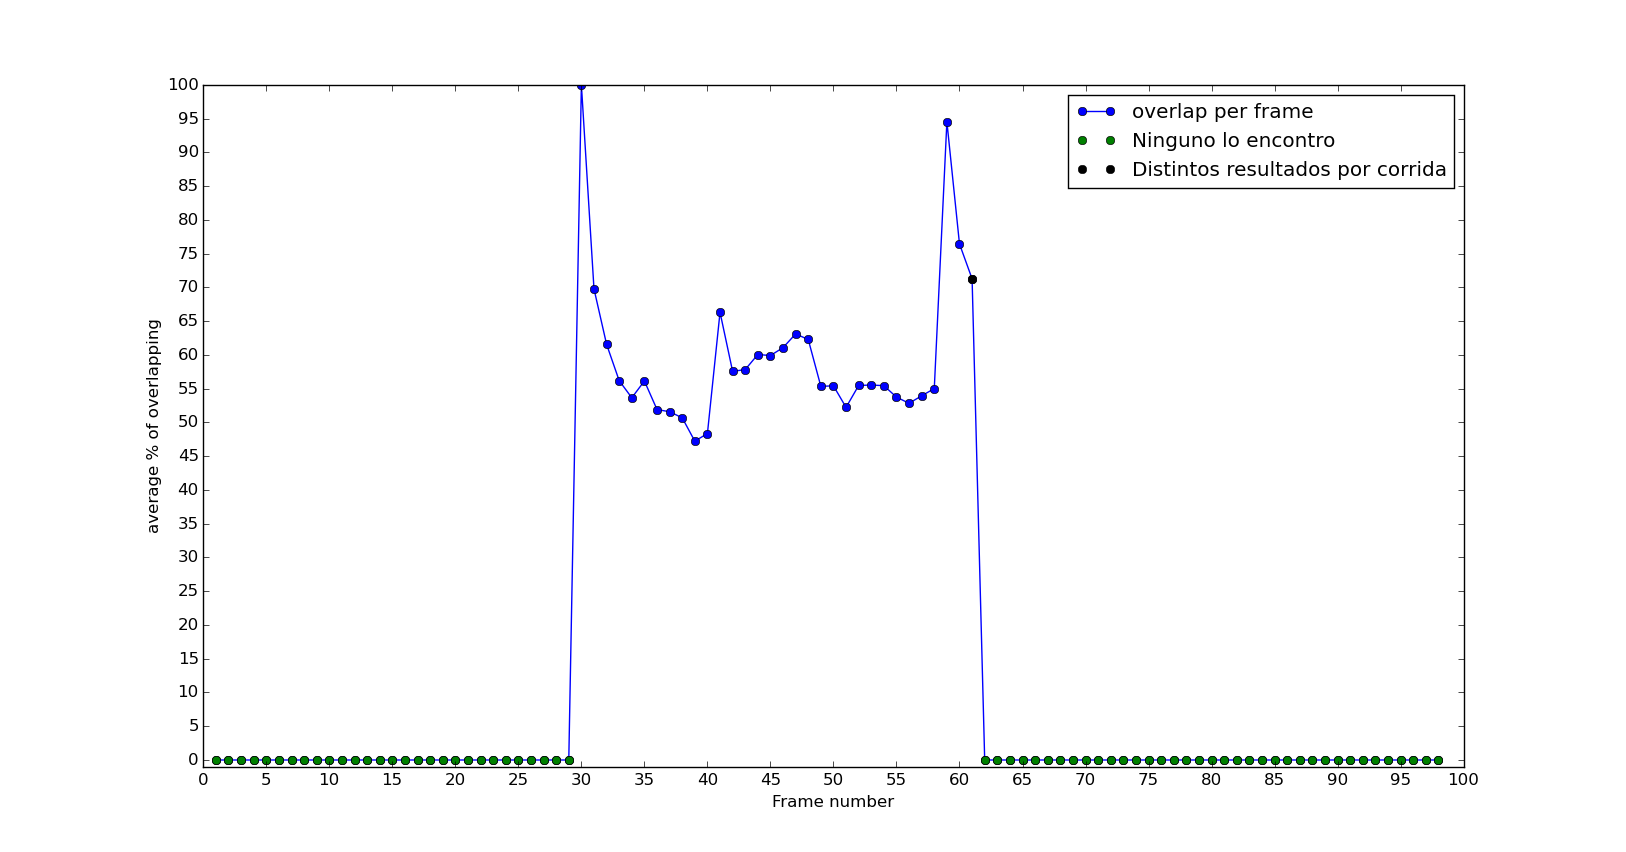
\includegraphics[width=\textwidth]{img/frame_a_frame/depth-gorra.png}
		\caption{Seguimiento frame a frame para la gorra}
		\label{frame_frame_d_gorra}
	\end{subfigure}
	\quad
	\begin{subfigure}[b]{\textwidth}
		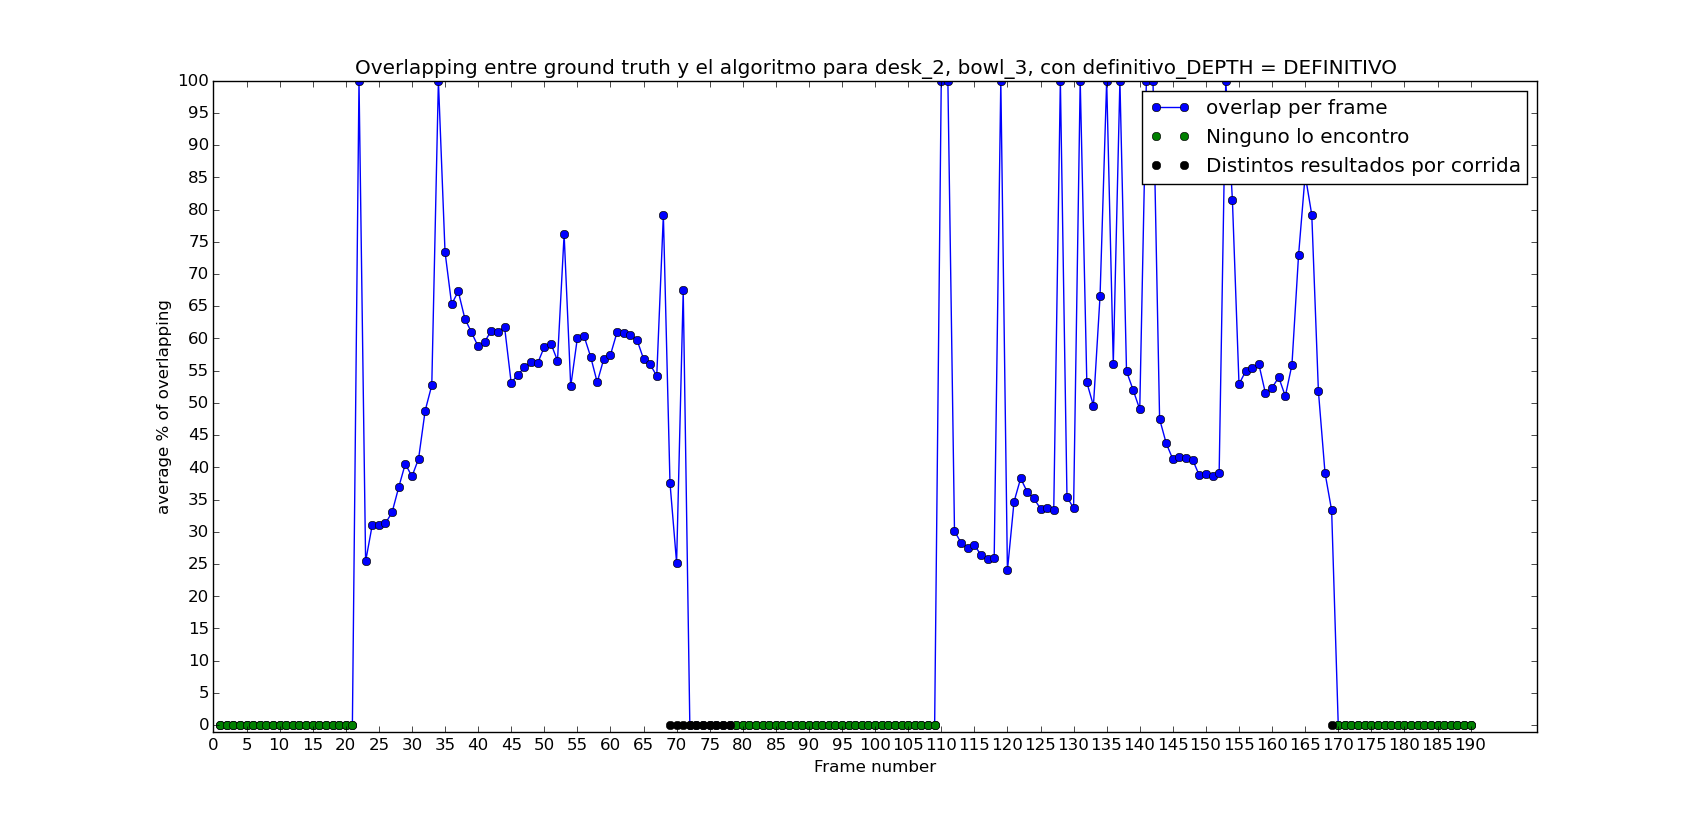
\includegraphics[width=\textwidth]{img/frame_a_frame/depth-bowl.png}
		\caption{Seguimiento frame a frame para el bowl}
		\label{frame_frame_d_bowl}
	\end{subfigure}
	\caption{Seguimiento frame a frame del tracking en profundidad con detección ideal.}
	\label{frame_frame_d}
\end{figure}


\subsection{Evaluación del tracking en RGB-D}
Una vez analizados el tracking RGB y Depth por separado decidimos unir ambos métodos y corroborar como se comporta el tracking combinado. Como se explicó en la sección \ref{metodo_rgbd} la combinación se hizo de dos maneras distintas por lo que en el análisis también distinguiremos cada una de las combinaciones por separado.

\customsubsubsection{Tracking RGB-D con preferencia en Depth}
\begin{table}[h]
    \begin{tabular}{|c|c|c|c|c|c|}
    \hline
    & \multirow{2}{2.4cm}{\% promedio de overlap} & \multirow{2}{2cm}{\% veces seguido} & \multirow{2}{1.6cm}{Falsos Positivos} & \multirow{2}{1.6cm}{\% Falsos Negativos}\\
	Objeto & & & &\\
    \hline
    Taza   & 65.07      & 90.05     & 0        &   1.7 \\
    \hline
    Gorra  & 42.83      & 90.82     & 0        &  1.02 \\
    \hline
    Bowl   & 42.88      & 68.54     & 1.75     &  11.4 \\
    \hline
    \end{tabular}
\caption{Resultados del tracking RGB-D utilizando la detección ideal, priorizando el tracking en Depth.}
\label{tabla_rgbd_d}
\end{table}

La primer combinación que analizaremos es la que le da prioridad al tracking en Depth y que utiliza el tracking RGB solo para intentar mejorar el resultado obtenido con Depth. En la Tabla \ref{tabla_rgbd_d} vemos como se modificaron los promedios de solapamiento con respecto a la Tabla \ref{tabla_d}. En el único caso que mejoró el promedio de solapamiento es el de la taza en donde mejoró poco menos de un 1\%. En los casos de la gorra y el bowl empeoraron cerca de un 8\% y un 4\% respectivamente. Sin embargo en los tres casos se mejoró el porcentaje de seguimiento, haciendo más eficiente a este método combinado. Además, en esta tabla también puede verse que en el caso del bowl disminuyó la cantidad de falsos positivos y falsos negativos en comparación con el tracking exclusivamente para Depth. En la Figura \ref{frame_frame_rgbd_d} se puede refinar el análisis de falsos positivos y falsos negativos hecho en la Tabla \ref{tabla_rgbd_d}.

\begin{figure}
	\centering
	\begin{subfigure}[b]{\textwidth}
		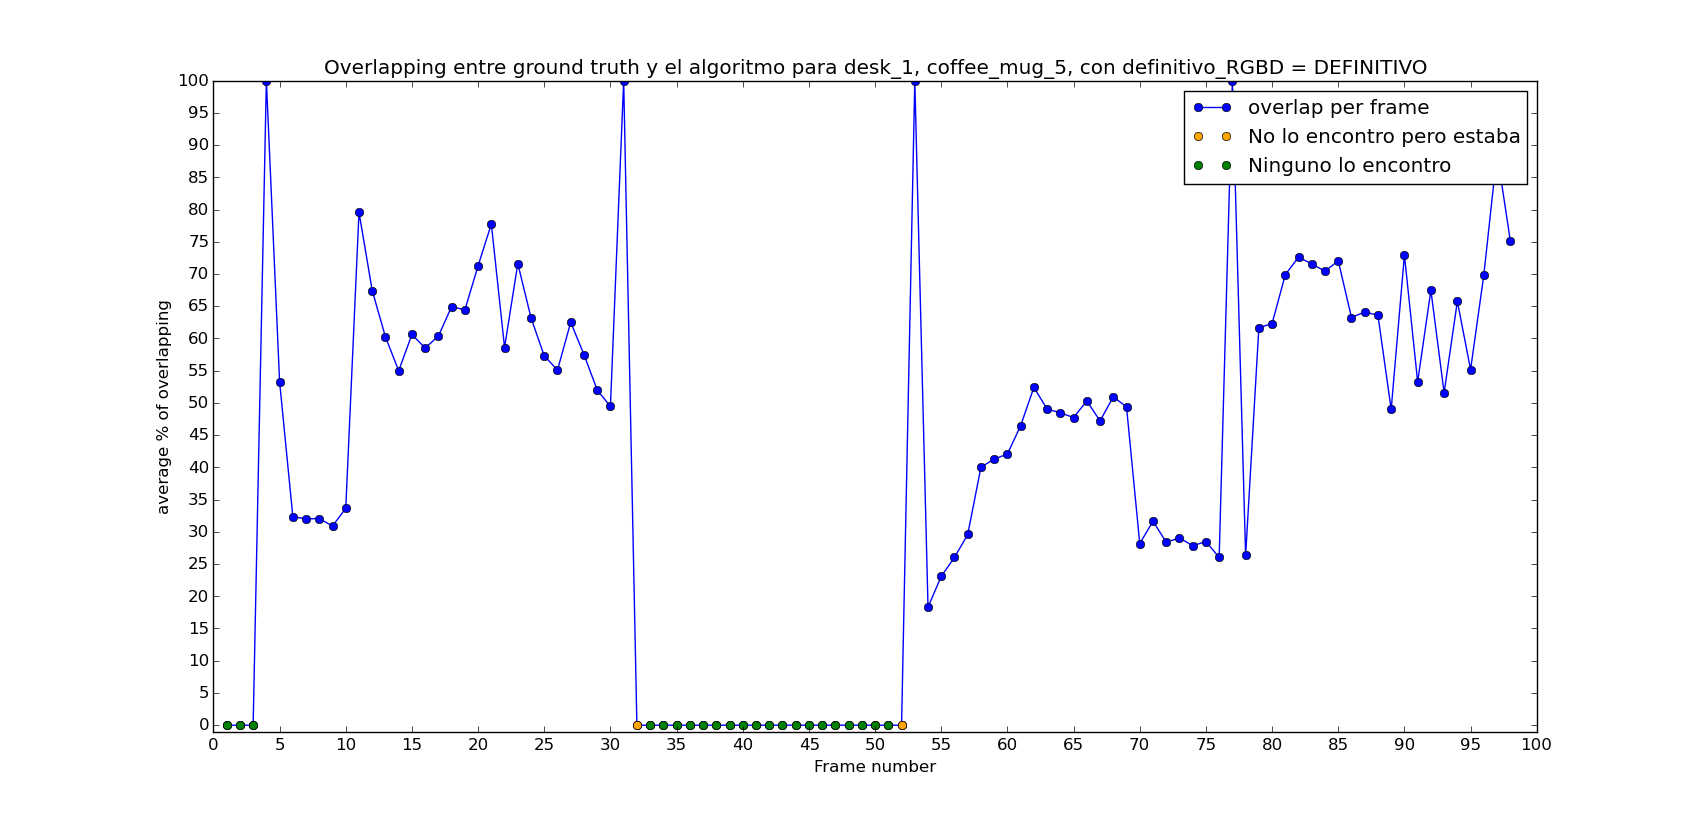
\includegraphics[width=\textwidth]{img/frame_a_frame/rgbd-d-taza.png}
		\caption{Seguimiento frame a frame para la taza}
		\label{frame_frame_rgbd_d_taza}
	\end{subfigure}
	\quad
	\begin{subfigure}[b]{\textwidth}
		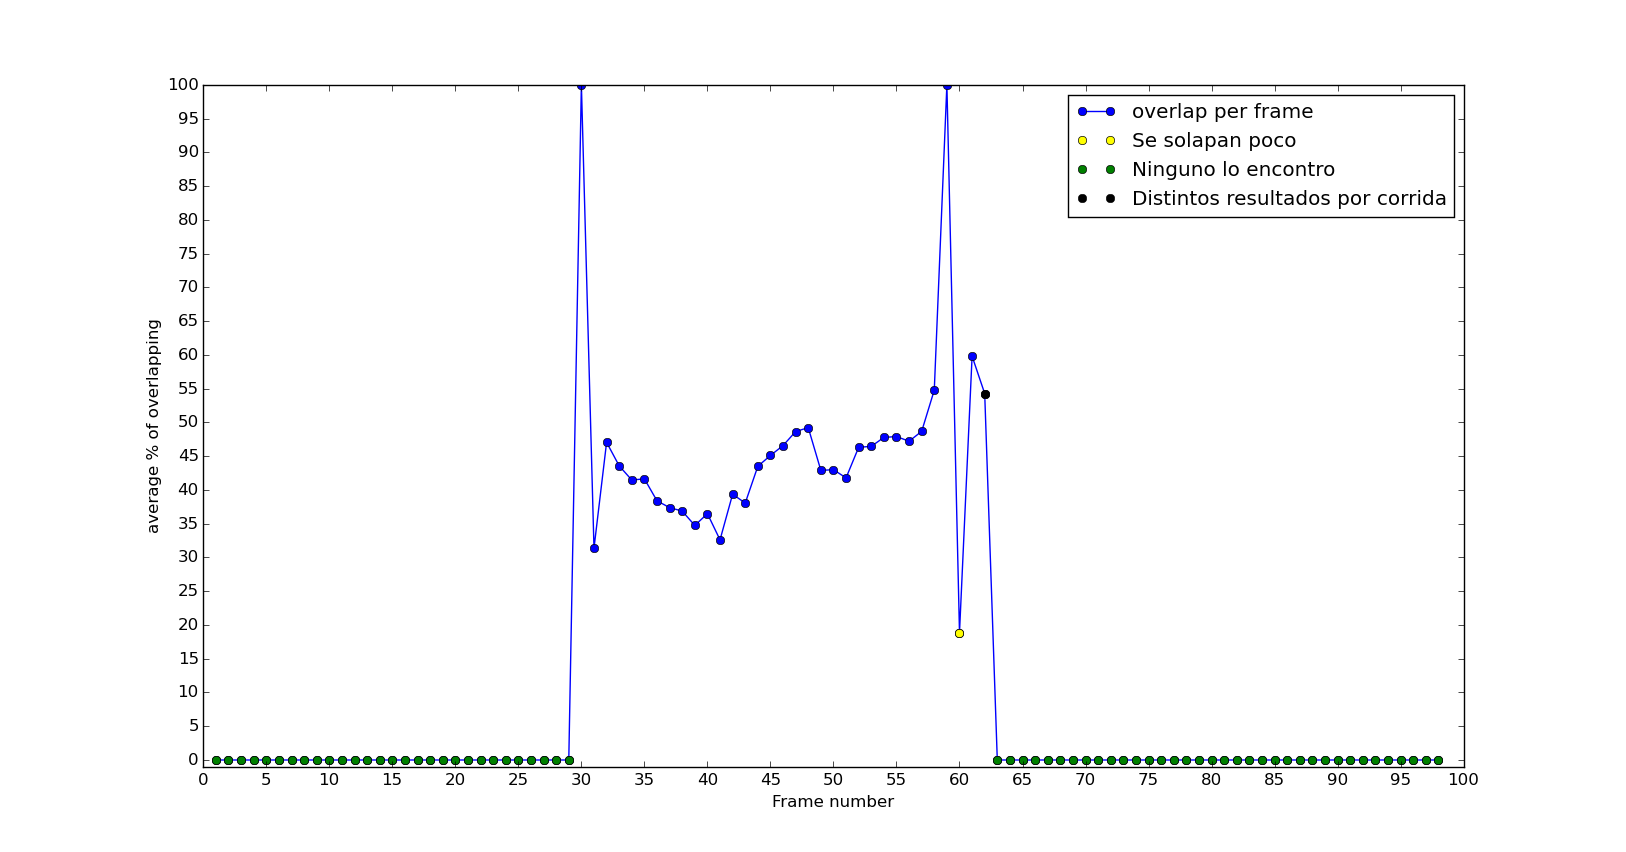
\includegraphics[width=\textwidth]{img/frame_a_frame/rgbd-d-gorra.png}
		\caption{Seguimiento frame a frame para la gorra}
		\label{frame_frame_rgbd_d_gorra}
	\end{subfigure}
	\quad
	\begin{subfigure}[b]{\textwidth}
		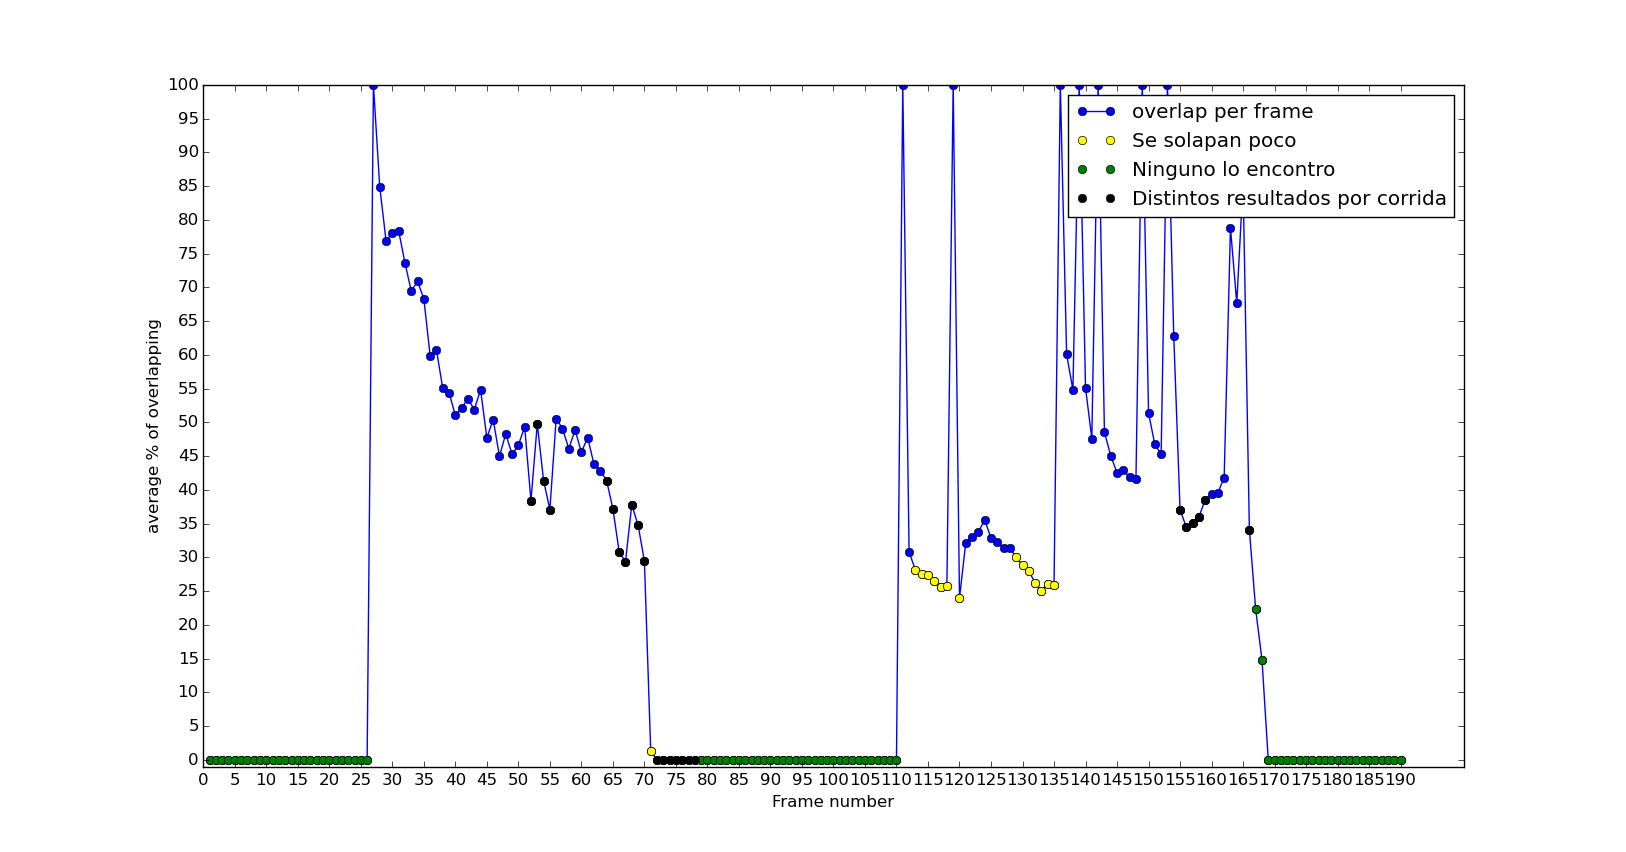
\includegraphics[width=\textwidth]{img/frame_a_frame/rgbd-d-bowl.png}
		\caption{Seguimiento frame a frame para el bowl}
		\label{frame_frame_rgbd_d_bowl}
	\end{subfigure}
	\caption{Seguimiento frame a frame para el tracking RGB-D con preferencia en profundidad usando la detección ideal.}
	\label{frame_frame_rgbd_d}
\end{figure}


Una hipótesis sobre la marcada diferencia del porcentaje de solapamiento entre el tracking RGB-D y Depth es la manera en que se hace la comparación de histogramas entre el área de búsqueda del frame actual y uno de los templates del objeto. \comentarioM{Ver frames 42, 57 de la primer corrida y frames 57, 58, 60 de la tercera}. Para esta comparación, como se explicó en la sección \ref{tracking_rgb}, se toma solo uno de los templates del objeto tomados en la etapa de entrenamiento junto a su correspondiente máscara. Para este template se calcula el histograma utilizando su máscara. Como la gorra es casi totalmente roja, el histograma RGB va a estar claramente marcado por la presencia del color rojo. En cambio, en el recuadro reportado por el tracking en Depth no solo aparece parte del objeto o, en el mejor de los casos, la totalidad del objeto sino que además se incluye parte del backround de la imagen. En la Figura \ref{mejora_rgb_en_tracking_rgbd} se pueden ver los distintos recuadros analizados por la mejora RGB, el recuadro del frame anterior y el template del objeto utilizado en la comparación. Se marca además cuál es el recuadro del frame actual elegido como el mejor según la comparación RGB. \comentarioP{Tratar de explicar mejor ya que Pachi me comentó "¿Cómo?" en este párrafo}

\begin{figure}
	%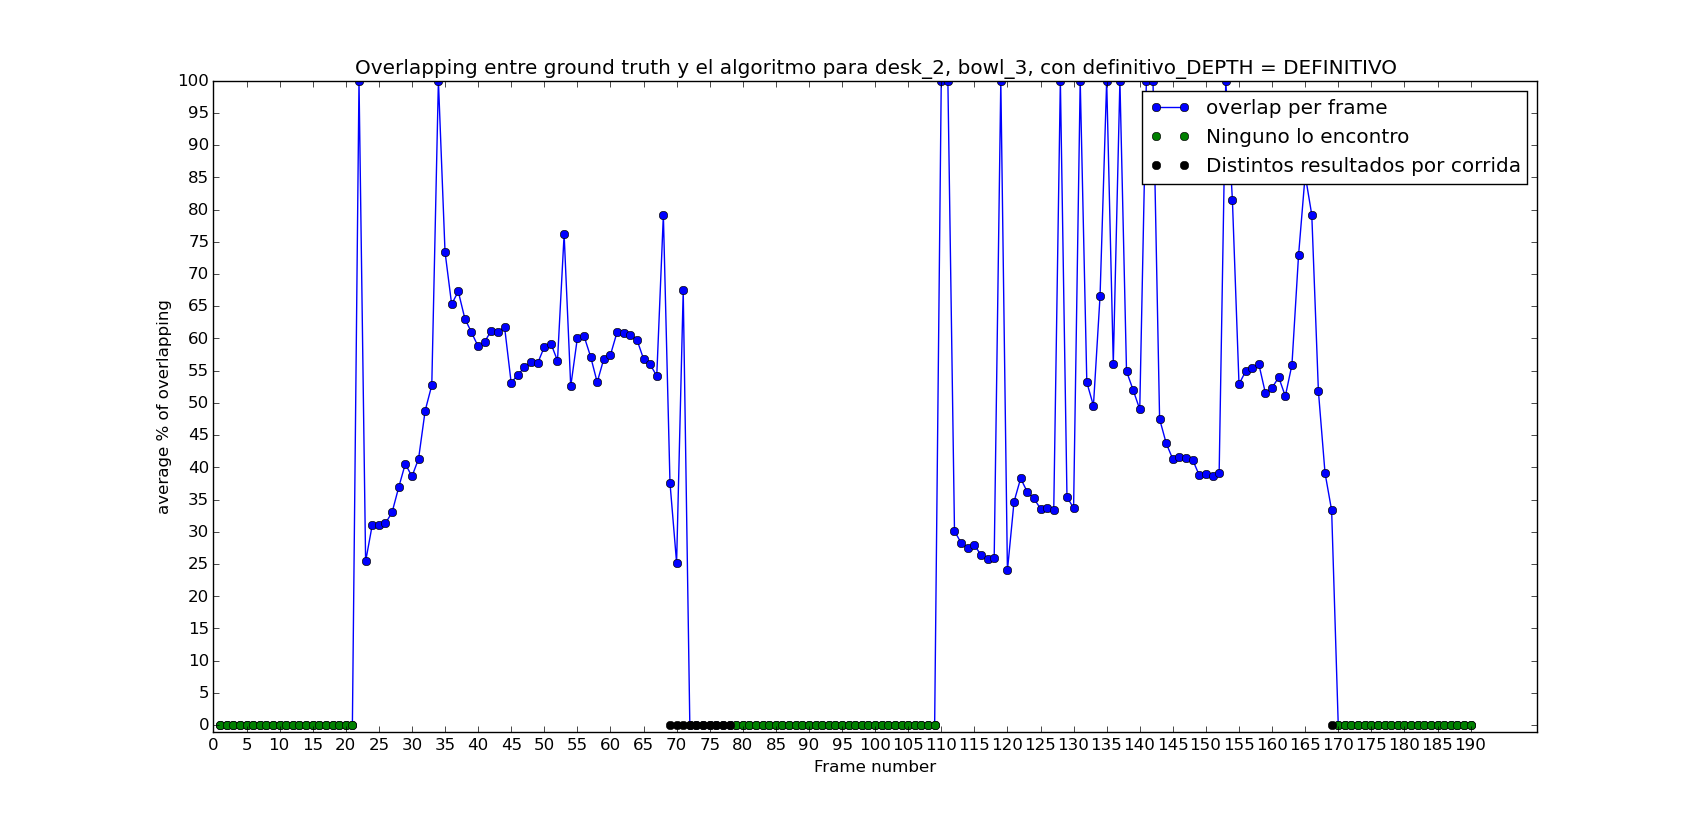
\includegraphics[width=\textwidth]{img/frame_a_frame/depth-bowl.png}
	\caption{Mejora obtenida según RGB para el tracking RGB-D}
	\label{mejora_rgb_en_tracking_rgbd}
\end{figure}

Una mejora para este algoritmo sería utilizar las máscaras tomadas durante el entrenamiento para calcular los histogramas de los recuadros del frame anterior y del actual. De esta manera, si la pose del objeto en estos recuadros coincide con alguna de las poses de los templates la comparación va a ser más robusta y permitiría evitar este tipo de inconvenientes en la mejora RGB.

\customsubsubsection{Tracking RGB-D con preferencia en RGB}
La segunda combinación para el tracking RGB-D es la que le da prioridad al tracking RGB e intenta mejorar el resultado utilizando el tracking Depth. Esta combinación se explica en detalle en la sección \ref{tracking_rgbd}.

\begin{table}[h]
    \begin{tabular}{|c|c|c|c|c|c|}
    \hline
    & \multirow{2}{2.4cm}{\% promedio de overlap} & \multirow{2}{2cm}{\% veces seguido} & \multirow{2}{1.6cm}{Falsos Positivos} & \multirow{2}{1.6cm}{\% Falsos Negativos}\\
	Objeto & & & &\\
    \hline
    Taza   & 50.48      & 83.10     & 0      & 8.16  \\
    \hline
    Gorra  & 63.91      & 96.94     & 0      & 0     \\
    \hline
    Bowl   & 13.39      &  6.87     & 0      & 13.33 \\
    \hline
    \end{tabular}
\caption{Resultados del tracking RGB-D utilizando la detección ideal, priorizando el tracking RGB.}
\label{tabla_rgbd_rgb}
\end{table}


Como se puede observar en la Tabla \ref{tabla_rgbd_rgb} y si se comparan los resultados con los de la Tabla \ref{tabla_rgb} podemos observar una notoria mejoría en la escena de la gorra. Para este objeto se mejoró casi un 13\% el promedio de solapamiento de áreas con un 2\% menos de desvío estándar casi sin variar el porcentaje de veces que se utilizó el tracking en toda la escena. Sin embargo el análisis para los otros dos objetos no varió mucho con respecto al seguimiento RGB.

Este resultado parece reafirmar la hipótesis hecha en la primer combinación RGB-D. En ese caso lo que vimos fue una baja importante en el porcentaje de solapamiento en comparación con el tracking en Depth para el caso de la gorra. Aquí parece suceder al revés: El algoritmo de seguimiento en RGB reporta un área pequeña dentro de la superficie de la gorra que se ve en la imagen RGB y a la hora de correr la mejora en Depth, esta trata de alinear la nube de puntos del frame anterior en la nube que proviene de tomar el resultado de RGB y proyectarlo en la escena en Depth. Como esta alineación es exitosa, el área reportada por el tracking en Depth proyectada en RGB es más grande que la reportada por el tracking RGB y por lo tanto se asemeja más a la indicada por el ground truth que contiene en el recuadro a la superficie de la gorra.




\subsection{Evaluación de los métodos de tracking en objetos desconocidos}
Las pruebas analizadas hasta el momento fueron todas realizadas con los mismos objetos y son estos los que se utilizaron durante la selección de métodos y luego la de parámetros. En esta sección se analizarán pruebas corridas con los métodos de las secciones anteriores pero utilizando objetos y escenas nuevas. Estas pruebas se realizaron con el objetivo de verificar el funcionamiento de los algoritmos en condiciones más realistas.

\begin{figure}
	\centering
	\begin{subfigure}[b]{0.3\textwidth}
		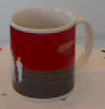
\includegraphics[width=\textwidth]{img/obj_nuevos/coffee_mug.png}
	\end{subfigure}
	\quad
	\begin{subfigure}[b]{0.3\textwidth}
		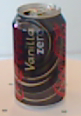
\includegraphics[width=\textwidth]{img/obj_nuevos/soda_can.png}
	\end{subfigure}
	\quad
	\begin{subfigure}[b]{0.3\textwidth}
		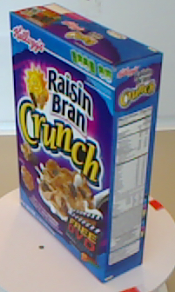
\includegraphics[width=\textwidth]{img/obj_nuevos/cereal_box.png}
	\end{subfigure}

	\begin{subfigure}[b]{0.3\textwidth}
		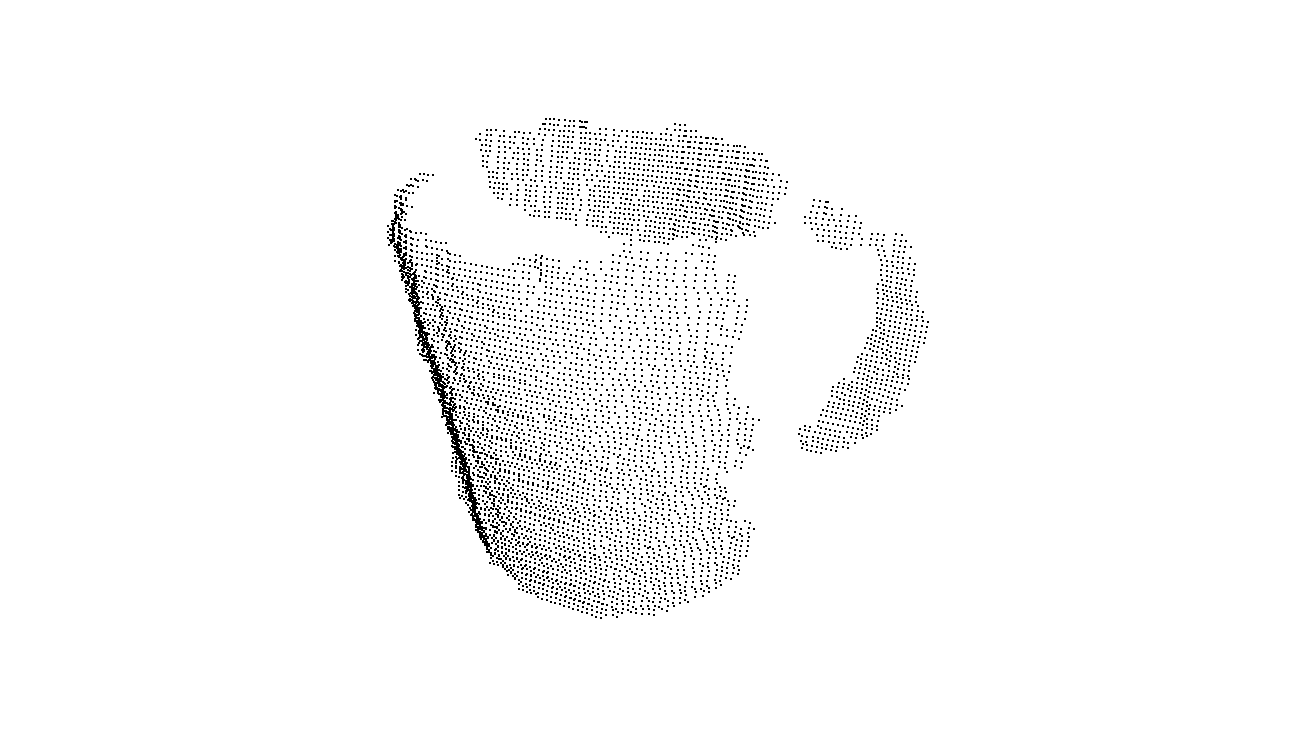
\includegraphics[width=\textwidth]{img/obj_nuevos/coffee_mug_pcd.png}
		\caption{Taza 2}
		\label{frame_frame_sistema-rgb-d_taza}
	\end{subfigure}
	\quad
	\begin{subfigure}[b]{0.3\textwidth}
		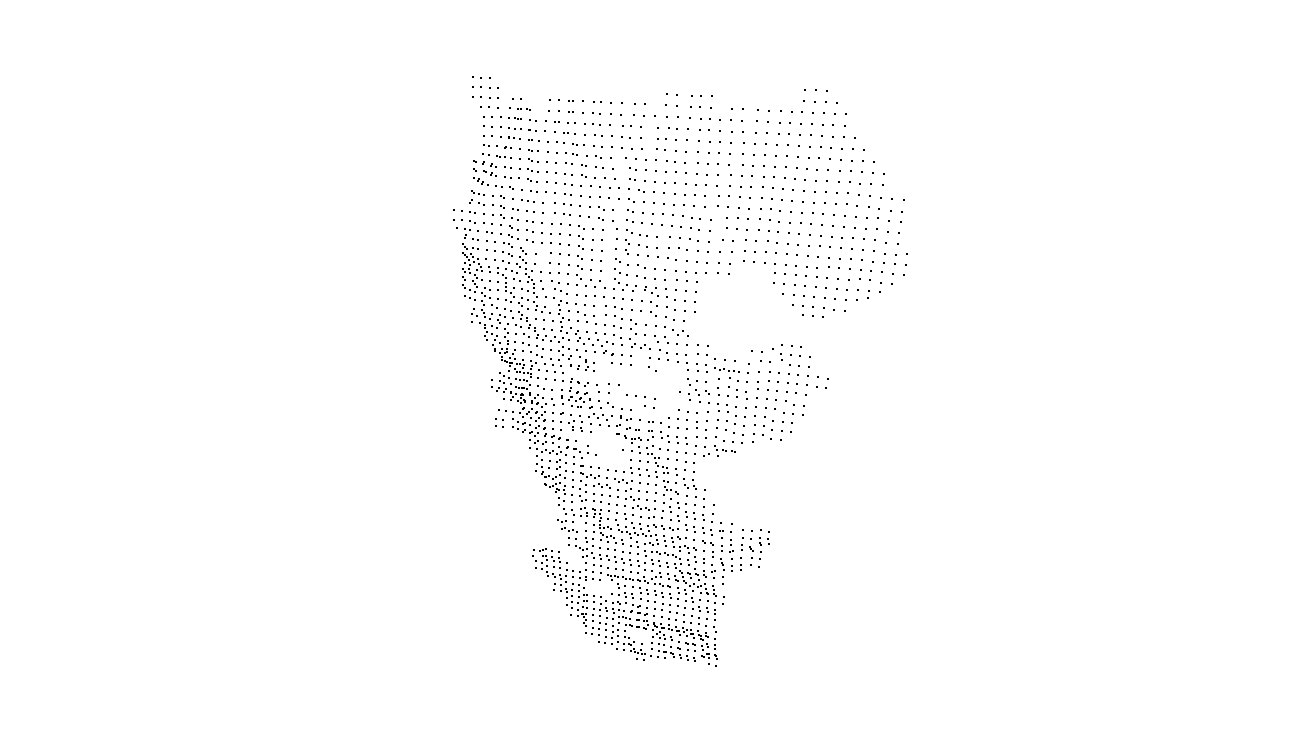
\includegraphics[width=\textwidth]{img/obj_nuevos/soda_can_pcd.png}
		\caption{Lata de gaseosa}
	\end{subfigure}
	\quad
	\begin{subfigure}[b]{0.3\textwidth}
		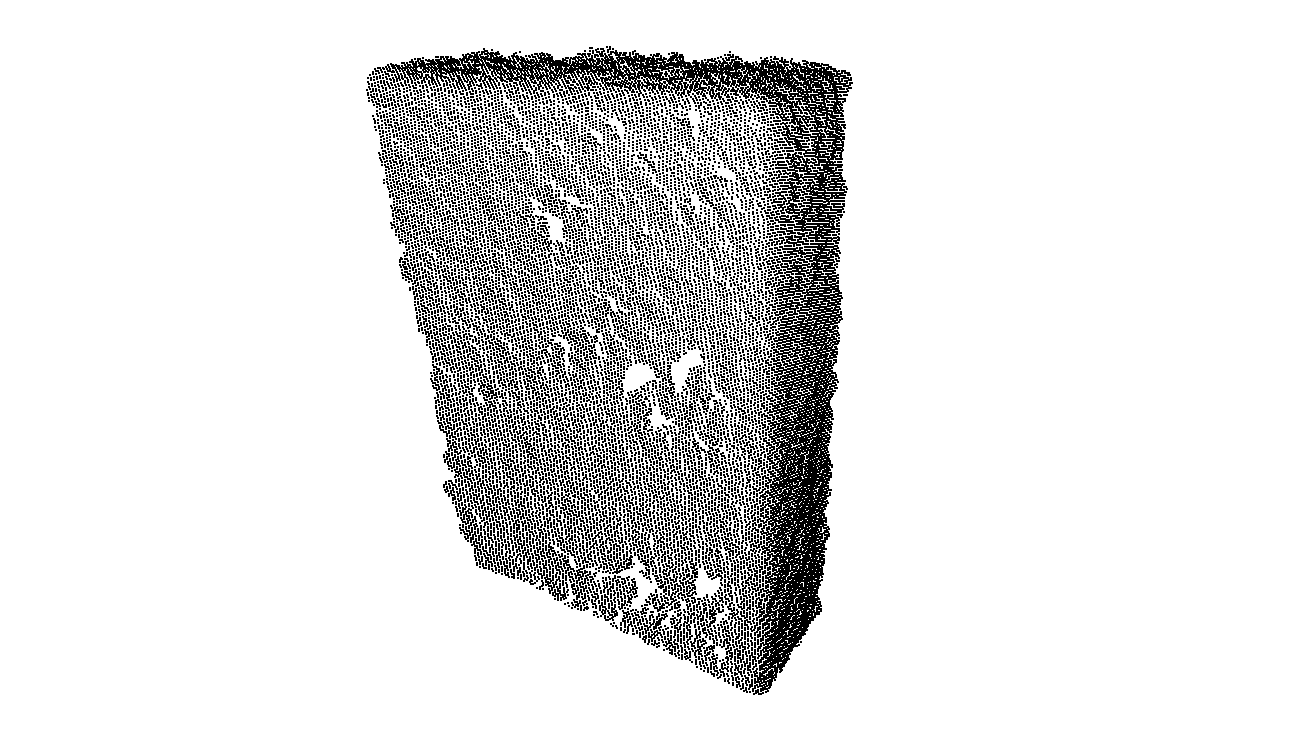
\includegraphics[width=\textwidth]{img/obj_nuevos/cereal_box_pcd.png}
		\caption{Caja de cereales}
	\end{subfigure}
	
	\caption{Objetos no utilizados durante las pruebas y selección de parámetros}
	\label{new_objects}
\end{figure}

Los objetos elegidos, que pueden verse en la Figura \ref{new_objects}, tienen distintas características y fueron elegidos bajo las siguientes hipótesis:
\begin{enumerate}
	\item Caja de cereales: al ser mayoritariamente plana debería perjudicar al tracking en Depth y por su textura bien definida beneficiar al tracking RGB
	\item Lata de gaseosa: posee una textura bien definida pero el fondo de la imagen es oscuro al igual que la lata por lo que debería perjudicar al tracking RGB
	\item Taza 2: es una taza diferente a la analizada antes. La forma debería beneficiar al tracking en Depth y sus colores a RGB.
\end{enumerate}

Las escenas anotadas en donde se utilizaron estos objetos para correr los algoritmos y evaluar su comportamiento son distintas a las usadas con los objetos anteriores. En este caso se usaron dos: una en donde predomina una mesa grande rectangular sobre una esquina de una habitación donde un lado está sobre una pared y el otro debajo de una ventana. En esta se encuentran entre otros objetos la lata y la taza 2. Se puede ver en la Figura \ref{escena_rgbd_base}. La otra también es sobre una mesa, pero esta vez es una mesa circular y pequeña en el centro de una habitación pegada sobre una columna. En esta escena es donde aparece la caja de cereales.


\begin{table}[h]
    \begin{tabular}{|c|c|c|c|c|c|}
    \hline
    & \multirow{2}{2.4cm}{\% promedio de overlap} & \multirow{2}{2cm}{\% veces seguido} & \multirow{2}{1.6cm}{Falsos Positivos} & \multirow{2}{1.6cm}{\% Falsos Negativos}\\
	Objeto & & & &\\
    \hline
    Taza 2  & 29.54      &  35.9     & 0        &  16 \\
    \hline
    Lata    &  0.01      &     0     & 12.8     &  52 \\
    \hline
    Caja    & 52.11      & 67.62     & 0        &   0 \\
    \hline
    \end{tabular}
\caption{Resultados del tracking RGB utilizando la detección ideal para objetos nuevos.}
\label{tabla_rgb_nuevos}
\end{table}


Teniendo en cuenta esta nueva selección de objetos y escenas y el motivo por el cual se eligió cada uno de ellos, analizaremos como se comportan los algoritmos en estos casos. En la Tabla \ref{tabla_rgb_nuevos} se pueden observar los resultados de estas pruebas. Como se esperaba, el algoritmo se comportó muy mal en el caso de la lata. Durante toda la escena el algoritmo reportó encontrar la lata en una zona que no se solapa con la reportada por el ground truth haciendo que el porcentaje de solapamiento sea muy bajo. En el caso de la nueva taza, el algoritmo funcionó de manera muy similar al caso de la taza que se utilizó durante el proceso de pruebas y selección de parámetros. En cuanto a la caja de cereales respecta, el algoritmo funcionó muy bien. A pesar del porcentaje relativamente bajo de veces que se siguió al objeto, las veces en las que hubo seguimiento el porcentaje de solapamiento fue bastante alto, como se puede ver en la Figura \ref{frame_frame_rgb_nuevo}. Un inconveniente que sufrió el algoritmo para esta escena es que la caja de cereales entre los frames 136 y 185 cambia la pose y en vez de estar de frente pasa a estar de costado. Esto provoca que el histograma que describe a la caja en esos frames cambie mucho con respecto al del template que está tomado de frente y de esta manera el seguimiento reporta no encontrar al objeto. Si no se tienen en cuenta esos frames, el porcentaje de veces que se utiliza el algoritmo de seguimiento pasaría a ser de un 89\%.

\begin{figure}
	\centering
	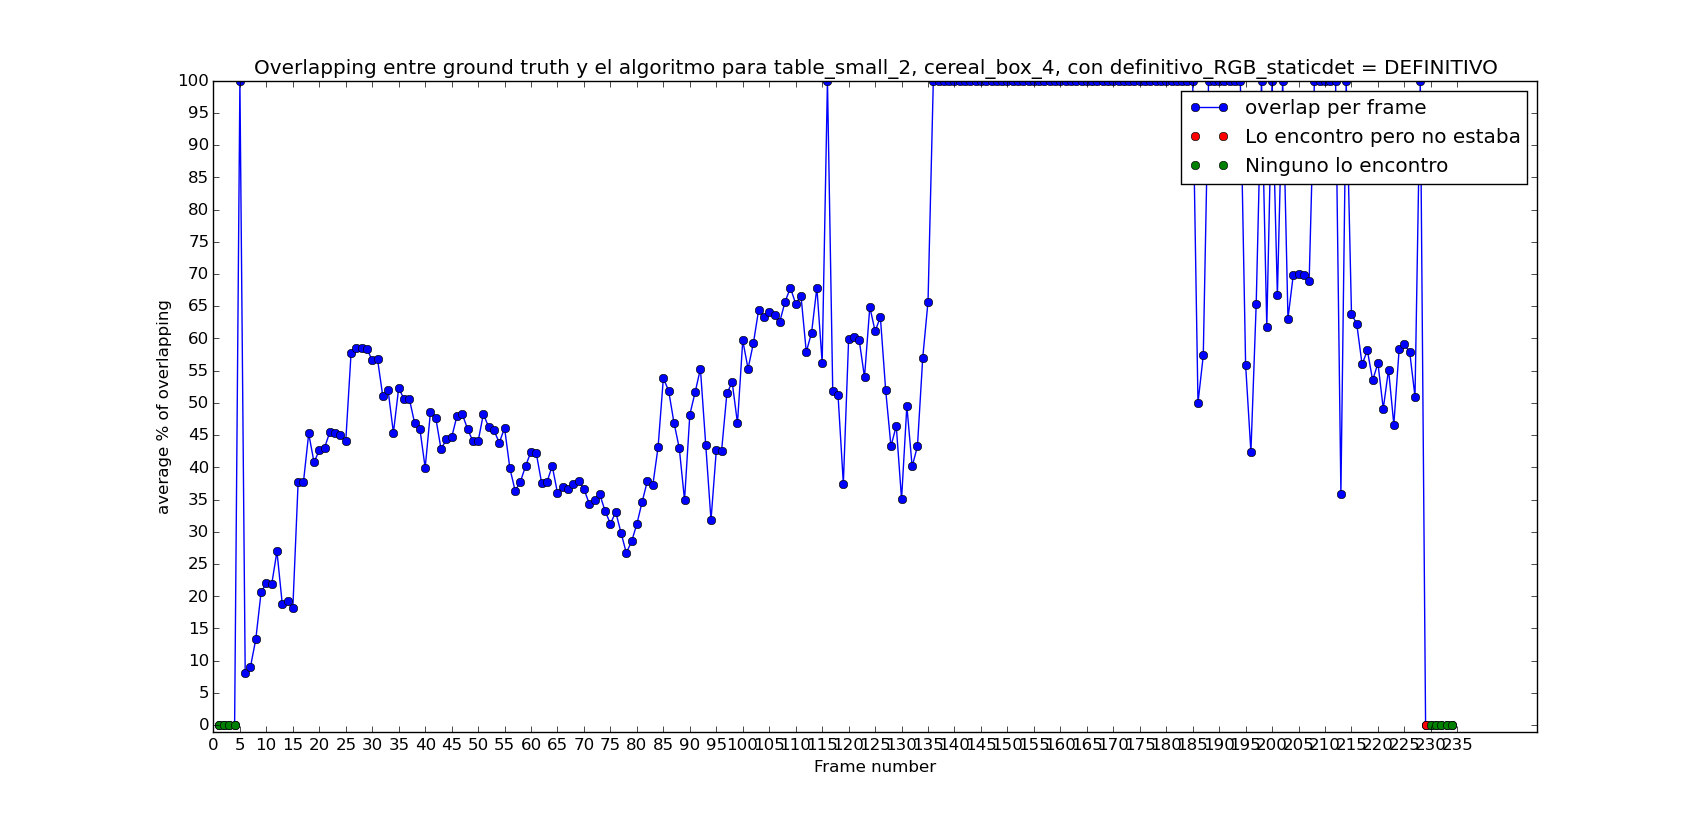
\includegraphics[width=\textwidth]{img/frame_a_frame/rgb-nuevo-caja.png}
	\caption{Seguimiento frame a frame para la caja de cereales según el tracking en RGB}
	\label{frame_frame_rgb_nuevo}
\end{figure}



\begin{table}[h]
    \begin{tabular}{|c|c|c|c|c|c|}
    \hline
    & \multirow{2}{2.4cm}{\% promedio de overlap} & \multirow{2}{2cm}{\% veces seguido} & \multirow{2}{1.6cm}{Falsos Positivos} & \multirow{2}{1.6cm}{\% Falsos Negativos}\\
	Objeto & & & &\\
    \hline
    Taza 2  & 55.79      & 80.51     & 0.27     &   1.2 \\
    \hline
    Lata    & 12.34      & 10.63     & 28.8     &    46 \\
    \hline
    Caja    & 44.94      & 30.62     & 0        & 11.97 \\
    \hline
    \end{tabular}
\caption{Resultados del tracking Depth utilizando la detección ideal para objetos nuevos.}
\label{tabla_d_nuevos}
\end{table}

En la Tabla \ref{tabla_d_nuevos} están los resultados del análisis del tracking en Depth para estos nuevos objetos. Para el ejemplo de la taza nueva el algoritmo se comporta de manera similar a la que lo hizo con la taza de las pruebas de selección de parámetros. En el caso de la lata los resultados fueron muy malos. El problema se debe a que en la primera detección indicada por el ground truth la taza apenas se aparecía en la nube de puntos de la escena. Esto hizo que la alineación del modelo fallara y que la nube de puntos resultante de esa detección sea casi por completo el plano de la mesa. Por este motivo el algoritmo alinea siempre ya que la mesa nunca sale del cuadro de la cámara.
Finalmente en el caso de la caja de cereales vemos que el algoritmo tiene un bajo porcentaje de veces que siguió al objeto. Si se observa la Figura \ref{frame_frame_d_nuevo}, debemos separar el análisis en tres partes. Por un lado, desde el inicio de la escena hasta el frame 136 el algoritmo funciona correctamente con un porcentaje de solapamiento promedio cercano al 45\% y una alta tasa de seguimiento. Luego, entre el frame 136 y el frame 185 sucede lo mismo que con el tracking RGB: el cambio de pose de la caja hace que el seguimiento falle y siempre se utilice la detección. Por último, entre el frame 185 y el fin de la escena el algoritmo vuelve a tener un buen porcentaje de solapamiento promedio y una tasa de seguimiento aceptable.

\begin{figure}
	\centering
	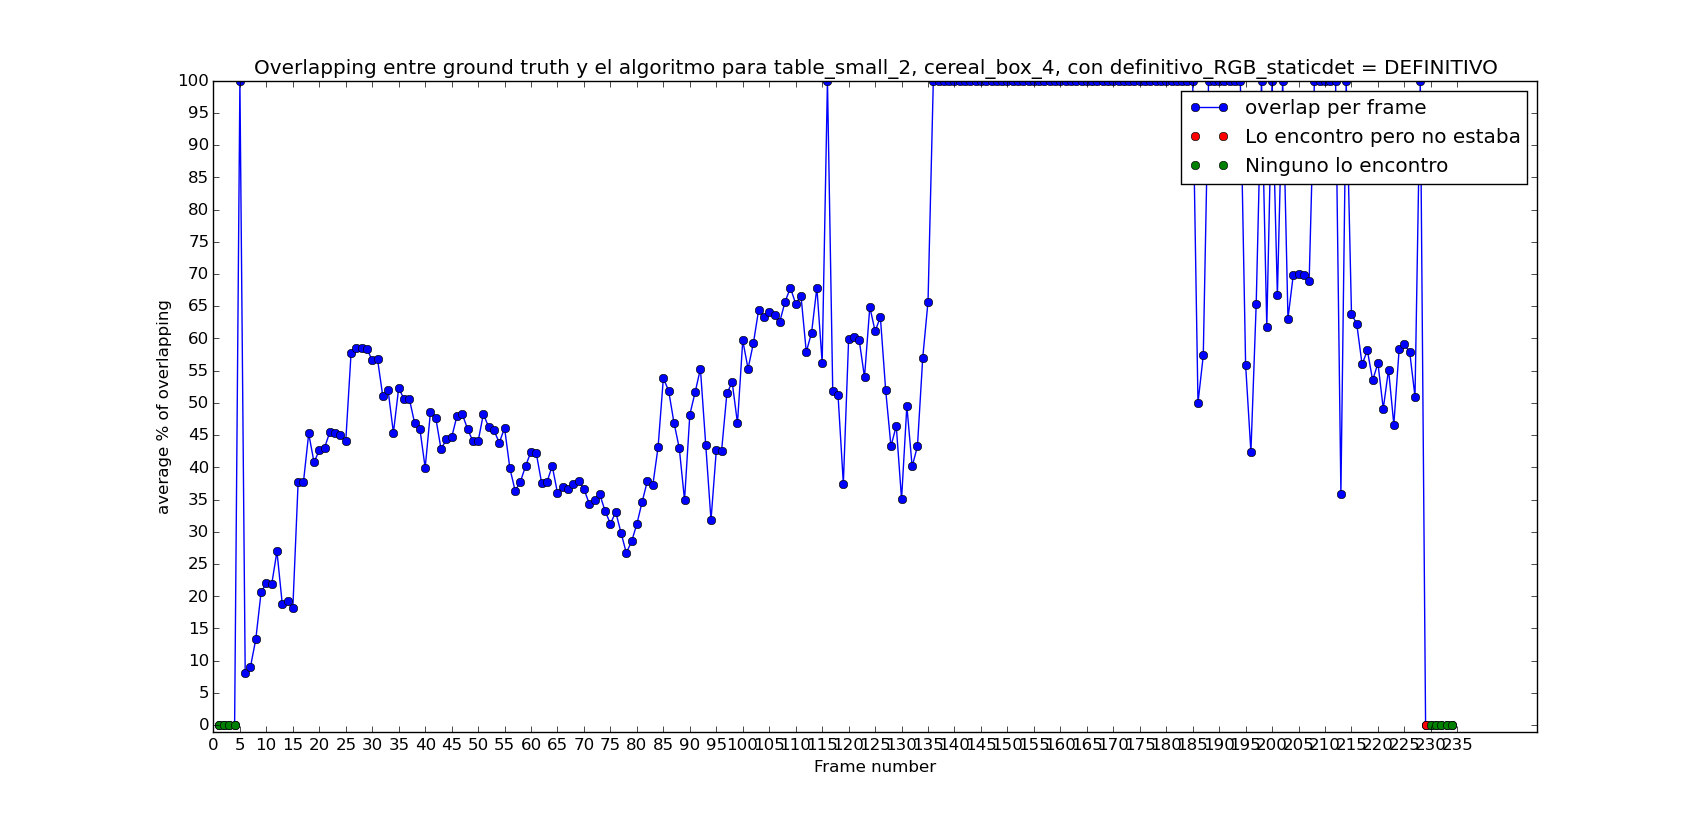
\includegraphics[width=\textwidth]{img/frame_a_frame/depth-nuevo-caja.png}
	\caption{Seguimiento frame a frame para la caja de cereales según el tracking en Depth}
	\label{frame_frame_d_nuevo}
\end{figure}


Finalmente analizamos los resultados de los algoritmos de tracking que combinan RGB con Depth. Estos pueden verse en las tablas \ref{tabla_rgbd_d_nuevos} y \ref{tabla_rgbd_rgb_nuevos}. En ambos casos los resultados son casi identicos a cada uno de los algoritmos por separado. Sólo se observan muy leves mejoras en la escena de la taza. \comentarioM{Después comento mas cosas.}\comentarioP{Falta decir que es mejor y cuando.}

\begin{table}[h]
    \begin{tabular}{|c|c|c|c|c|c|}
    \hline
    & \multirow{2}{2.4cm}{\% promedio de overlap} & \multirow{2}{2cm}{\% veces seguido} & \multirow{2}{1.6cm}{Falsos Positivos} & \multirow{2}{1.6cm}{\% Falsos Negativos}\\
	Objeto & & & &\\
    \hline
    Taza 2  & 35.98      & 48.33      & 0.8     & 10.93 \\
    \hline
    Lata    & 18.81      & 23.67      & 29.33   & 37.07 \\
    \hline
    Caja    & 35.03      & 23.29      & 0       & 16.67 \\
    \hline
    \end{tabular}
\caption{Resultados del tracking RGB-D con preferencia en Depth para objetos nuevos.}
\label{tabla_rgbd_d_nuevos}
\end{table}

\begin{table}[h]
    \begin{tabular}{|c|c|c|c|c|c|}
    \hline
    & \multirow{2}{2.4cm}{\% promedio de overlap} & \multirow{2}{2cm}{\% veces seguido} & \multirow{2}{1.6cm}{Falsos Positivos} & \multirow{2}{1.6cm}{\% Falsos Negativos}\\
	Objeto & & & &\\
    \hline
    Taza 2  & 33.62      & 39.32      & 0       & 14.93\\
    \hline
    Lata    &  0.01      &     0      & 12.8    &  52.0\\
    \hline
    Caja    & 52.11      & 67.62      & 0       &     0\\
    \hline
    \end{tabular}
\caption{Resultados del tracking RGB-D con preferencia en RGB y detección ideal para objetos nuevos.}
\label{tabla_rgbd_rgb_nuevos}
\end{table}



\subsection{Evaluación del sistema RGB-D}
Para finalizar con la evaluación de los métodos, presentamos en esta sección los resultados para todas las escenas antes vistas correspondientes al sistema RGB-D explicado en la sección \ref{metodo_rgbd}.

\begin{table}[h]
    \begin{tabular}{|c|c|c|c|c|c|}
    \hline
    & \multirow{2}{2.4cm}{\% promedio de overlap} & \multirow{2}{2cm}{\% veces seguido} & \multirow{2}{1.6cm}{Falsos Positivos} & \multirow{2}{1.6cm}{Falsos Negativos}\\
	Objeto & & & & & Accuracy\\
	\hline
    Taza    & 50.44      & 76.67     &    0           & 16.67    & 0.83 \\
    \hline
    Gorra   & 50.05      & 68.09     &    0           &  10.2    & 0.9 \\
    \hline
    Bowl    & 28.18      & 45.67     &    0           &  28.6    & 0.71 \\
    \hline
    Taza 2  & 45.54      & 77.78     &    0           &  6.93    & 0.93 \\
    \hline
    Lata    & 12.72      & 25.85     &   20           & 40.53    & 0.39 \\
    \hline
    Caja    &  6.17      &    10     &    0           & 73.08    & 0.27 \\
    \hline
    \end{tabular}
\caption{Resultados del sistema de seguimiento RGB-D}
\label{tabla_sistema_rgbd}
\end{table}

En la Tabla \ref{tabla_sistema_rgbd} se puede ver un análisis similar al realizado anteriormente para cuantificar el comportamiento de los algoritmos de tracking. La principal diferencia es que en esta tabla se incluyen los resultados de las detecciones para el promedio de solapamiento y para el porcentaje de veces seguido, ya que en esta ocasión las detecciones son automáticas y por lo tanto nos interesa conocer el comportamiento del sistema de seguimiento en su totalidad. Además, se incluye el \textit{accuracy} como medida de cuantificación. El \textit{accuracy} es la proporción de resultados correctos sobre el total de los casos examinados. Su fórmula es la siguiente:
\begin{equation}
\frac{\#true\_positives + \#true\_negatives}{\#true\_positives + \#true\_negatives + \#false\_positives + \#false\_negatives}
\end{equation}

Como podemos ver, en las corridas de las dos tazas y la gorra el accuracy es alto, entre 0.83 y 0.93. Esto significa que en el 83\% o 93\% de los frames el algoritmo reportó correctamente la ubicación del objeto. Además, en estos tres ejemplos el promedio de porcentaje de solapamiento está por encima del 45\% y el porcentaje de seguimiento por encima del 71\%.

Si comparamos los resultados del sistema con los resultados de cada método de seguimiento por separado usando la detección ideal vemos como nuestro sistema responde muy bien y en muchos casos superando a los otros métodos.

El seguimiento en RGB con detección ideal supera al sistema en el caso de la gorra, en la cual el porcentaje promedio de solapamiento es un 5\% mejor que el sistema y cerca de 30\% más de porcentaje de seguimiento. Creemos que esto se debe a la combinación de un modelo de nube de puntos de la gorra malo y el método de detección que resulta poco robusto. También es mejor en el caso de la caja de cereales, superando en un 50\% tanto al porcentaje de solapamiento como al de veces que se siguió al objeto. En parte esto sucede por motivos similares al de la gorra, sumando que sobre la mitad de la escena y casi hasta el final, la caja queda de perfil a la cámara haciendo que el modelo 3D de la misma no sirva para alinearlo con la escena y por lo tanto empeorando mucho el rendimiento. Sin embargo en el resto de las escenas, específicamente para ambas tazas, el bowl y la lata, el sistema supera ampliamente no solo al porcentaje de solapamiento promedio sino también al porcentaje de veces que se sigue al objeto y el porcentaje de falsos positivos.

En el caso del seguimiento en profundidad se nota cómo un buen método de detección, en este caso el método ideal, beneficia al algoritmo de seguimiento. Si comparamos los resultados de las tablas \ref{tabla_d} y \ref{tabla_d_nuevos} del tracking en profundidad con los de la Tabla \ref{tabla_sistema_rgbd} del sistema RGB-D vemos que en la mayoría de los casos el seguimiento en profundidad con detección ideal supera ampliamente al sistema RGB-D en porcentaje de seguimiento y por bastante también en porcentaje promedio de solapamiento. Sólo en el ejemplo de la lata el sistema se comporta mejor. Sin embargo, el sistema demuestra ser mucho más robusto que el tracking en profundidad ya que mejora en todos los casos el porcentaje de falsos positivos.

A continuación presentamos los gráficos de seguimiento frame a frame para el sistema RGB-D de las escenas de la taza, la gorra y el bowl.

\begin{figure}
	\centering
	\begin{subfigure}[b]{\textwidth}
		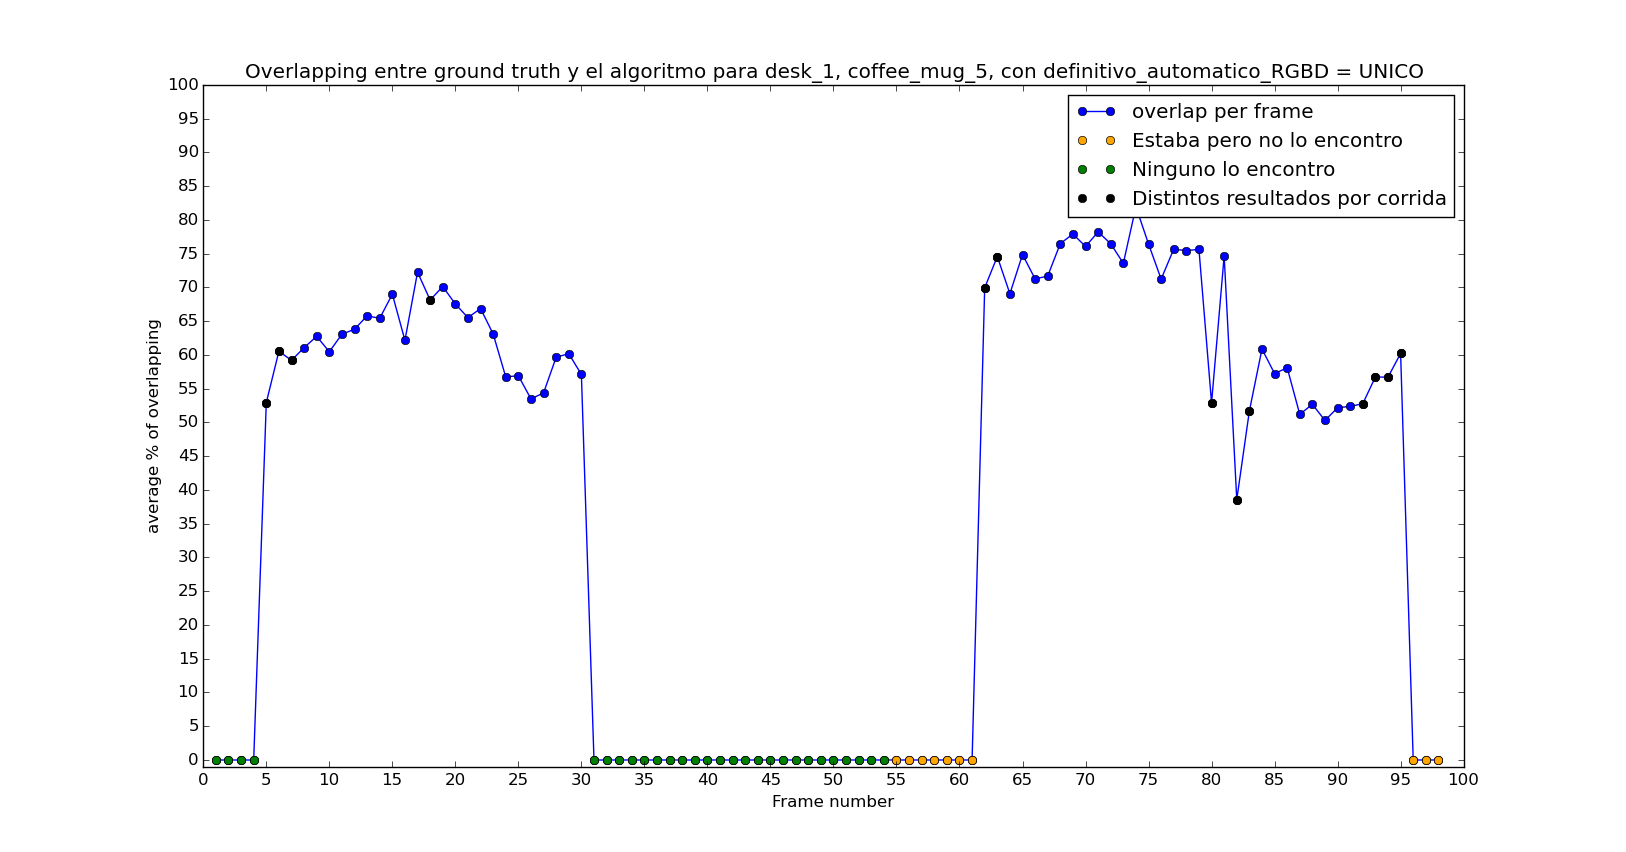
\includegraphics[width=\textwidth]{img/frame_a_frame/sistema-rgbd-taza.png}
		\caption{Seguimiento frame a frame para la taza}
		\label{frame_frame_sistema-rgb-d_taza}
	\end{subfigure}
	\quad
	\begin{subfigure}[b]{\textwidth}
		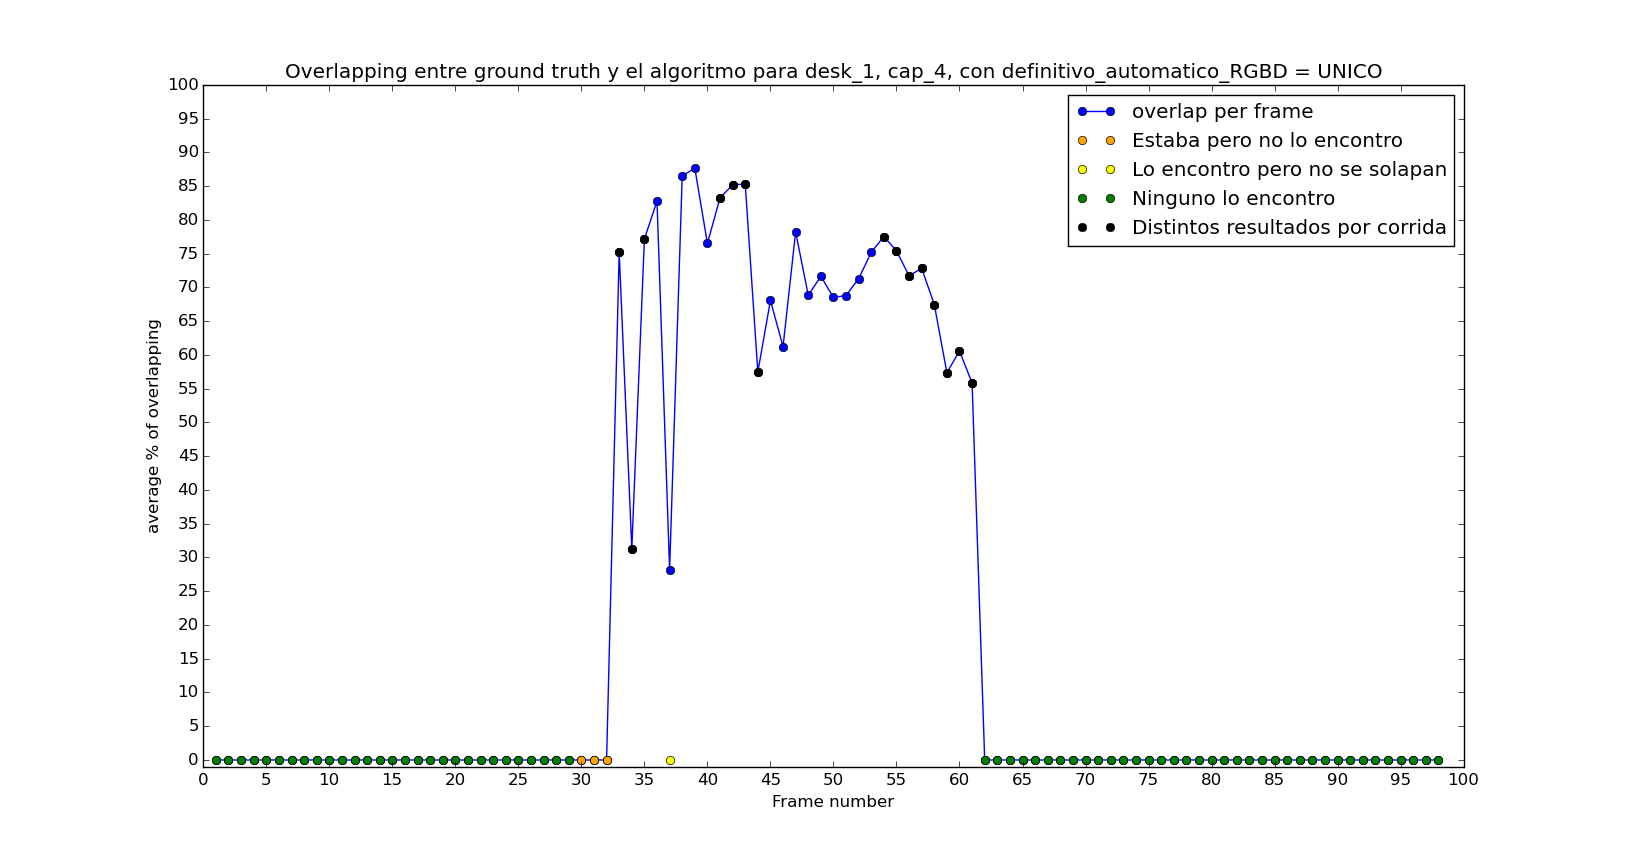
\includegraphics[width=\textwidth]{img/frame_a_frame/sistema-rgbd-gorra.png}
		\caption{Seguimiento frame a frame para la gorra}
		\label{frame_frame_sistema-rgb-d_gorra}
	\end{subfigure}
	\quad
	\begin{subfigure}[b]{\textwidth}
		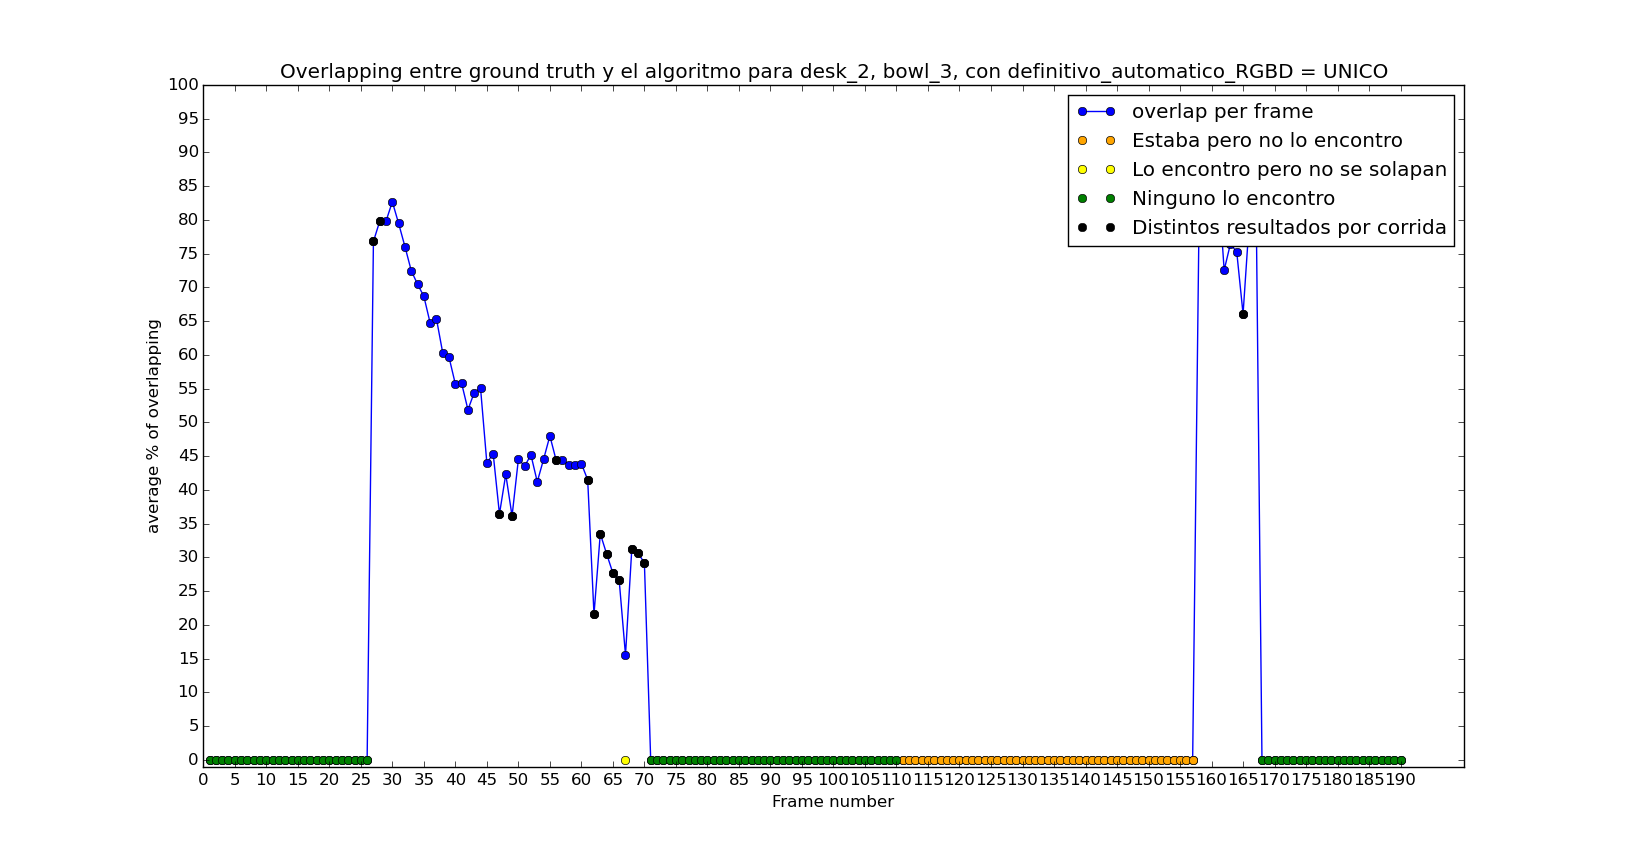
\includegraphics[width=\textwidth]{img/frame_a_frame/sistema-rgbd-bowl.png}
		\caption{Seguimiento frame a frame para el bowl}
		\label{frame_frame_sistema-rgb-d_bowl}
	\end{subfigure}
	\caption{Seguimiento frame a frame del sistema RGB-D}
	\label{frame_frame_d}
\end{figure}






\comentarioP{Falta decir que es mejor y cuando}

\section{Discusión}
